% SPDX-FileCopyrightText: 2025 Jorge Teixeira Crespo <jorge.teixeira@udc.es>
%
% SPDX-License-Identifier: GPL-2.0-or-later

\chapter{State of the Art}
\label{chap:state-of-the-art}

\lettrine{T}{he} following sections survey the principal technical options for each core service GPUL operates or is expected to adopt in the near future.  
For every category an introduction explains its relevance, followed by one \emph{Current stack} subsection and a set of numbered subsections that describe the state of the art.  

%--------------------------------------------------------------------
\section{Mailing-list Managers}

\textbf{Importance.} Mailing lists are a foundational tool for formal communication, providing a standardized and archivable channel for discussions and announcements. For community-driven associations, they are crucial for transparent decision-making and record-keeping. This is especially true for GPUL, as its statutes explicitly name mailing lists as the official communication channel. Consequently, the service must be reliable, searchable, and permanently archived to preserve organizational history and ensure newcomers can access past discussions.

\subsection*{Current stack}
\textbf{Mailman 2} running on Debian 8 (see Figure~\ref{fig:mailman2}).

\begin{figure}[H]
  \centering
  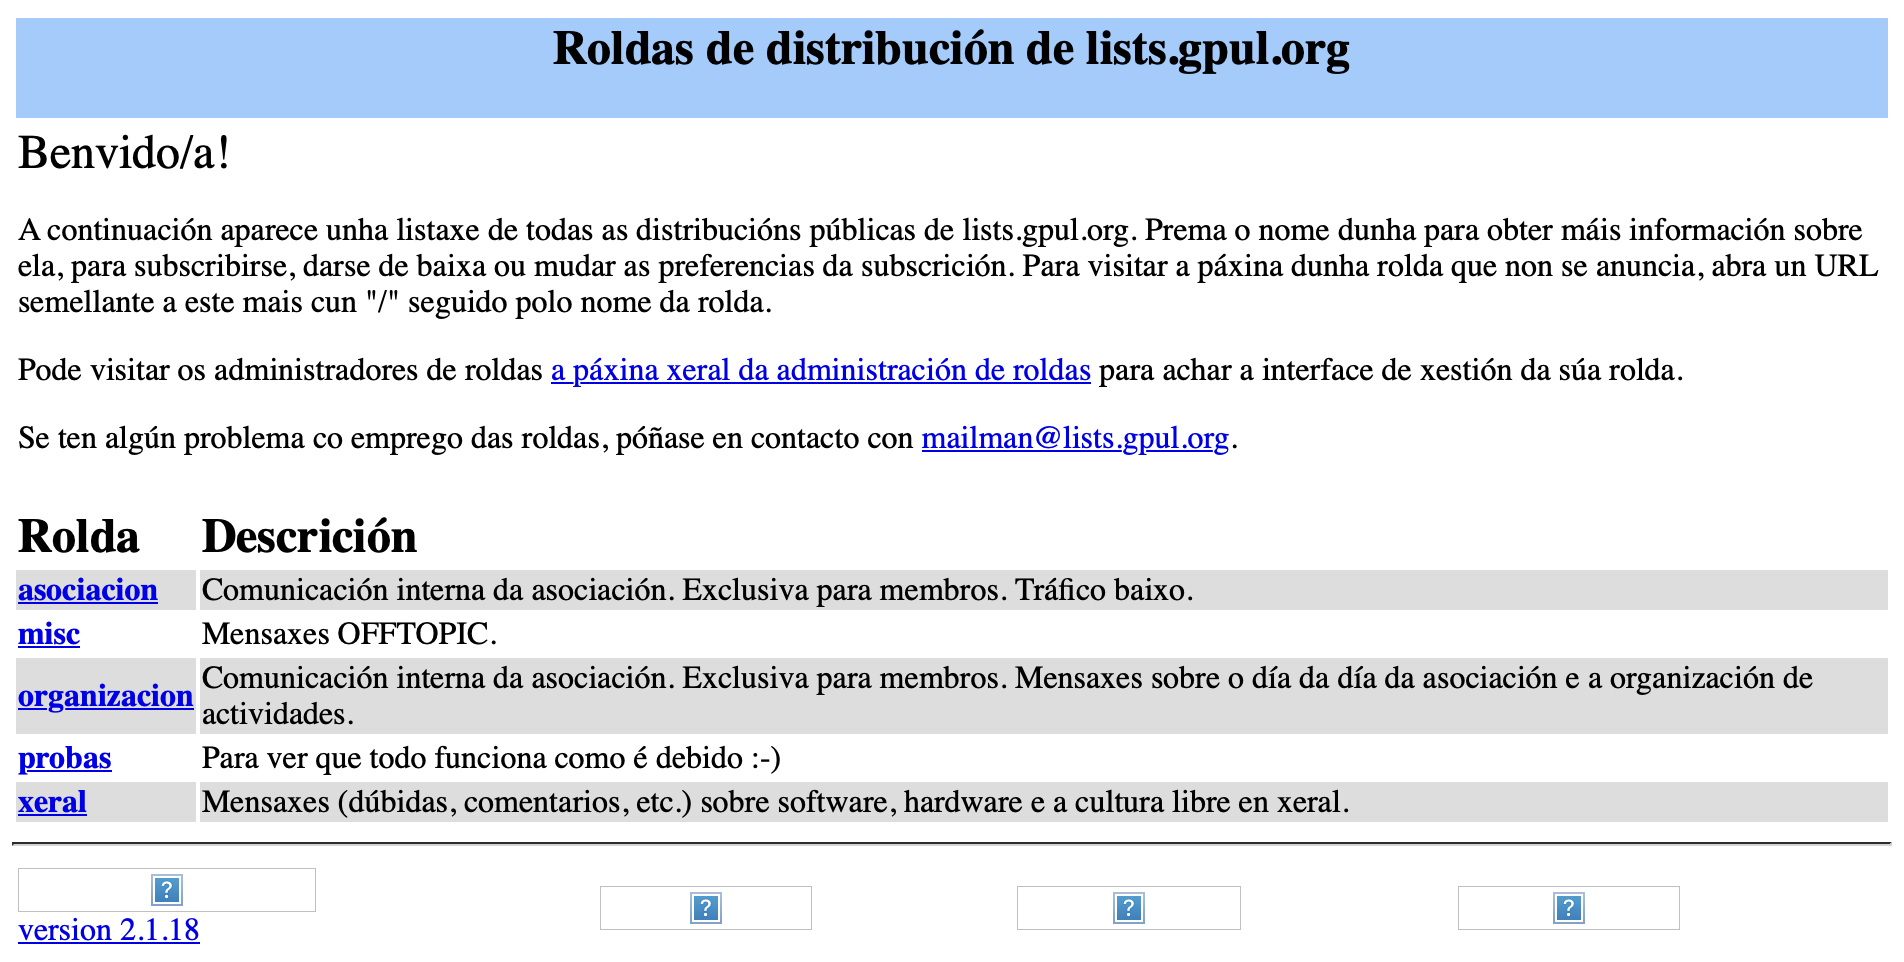
\includegraphics[width=0.9\textwidth]{imaxes/mailman-2-current.png}
  \caption{Current Mailman 2 interface}
  \label{fig:mailman2}
\end{figure}

\subsection*{Mailman 3 + HyperKitty}

Mailman~3 is a modular mailing list management system, described in its official documentation~\cite{mailman-install-docs}. It is the modern successor to the Mailman~2 software currently in use, and includes official migration tools to assist in upgrading existing lists and archives. Its core component, Mailman Core, is responsible for all mailing list logic and message delivery. It communicates with a Mail Transfer Agent (MTA) via \gls{lmtp} for incoming messages and \gls{smtp} for outgoing ones, and exposes a \gls{restapi} for external interfaces.

HyperKitty~\cite{hyperkitty-docs} is the web-based archiver of Mailman~3, designed to replace Pipermail. It receives messages from Mailman Core through the \texttt{mailman-hyperkitty} plugin and indexes them into a database. The messages are then accessible via a modern web interface that allows browsing, searching, and replying to threads. A screenshot of the HyperKitty interface is shown in Figure~\ref{fig:fedora-hyperkitty}.

\begin{figure}[H]
  \centering
  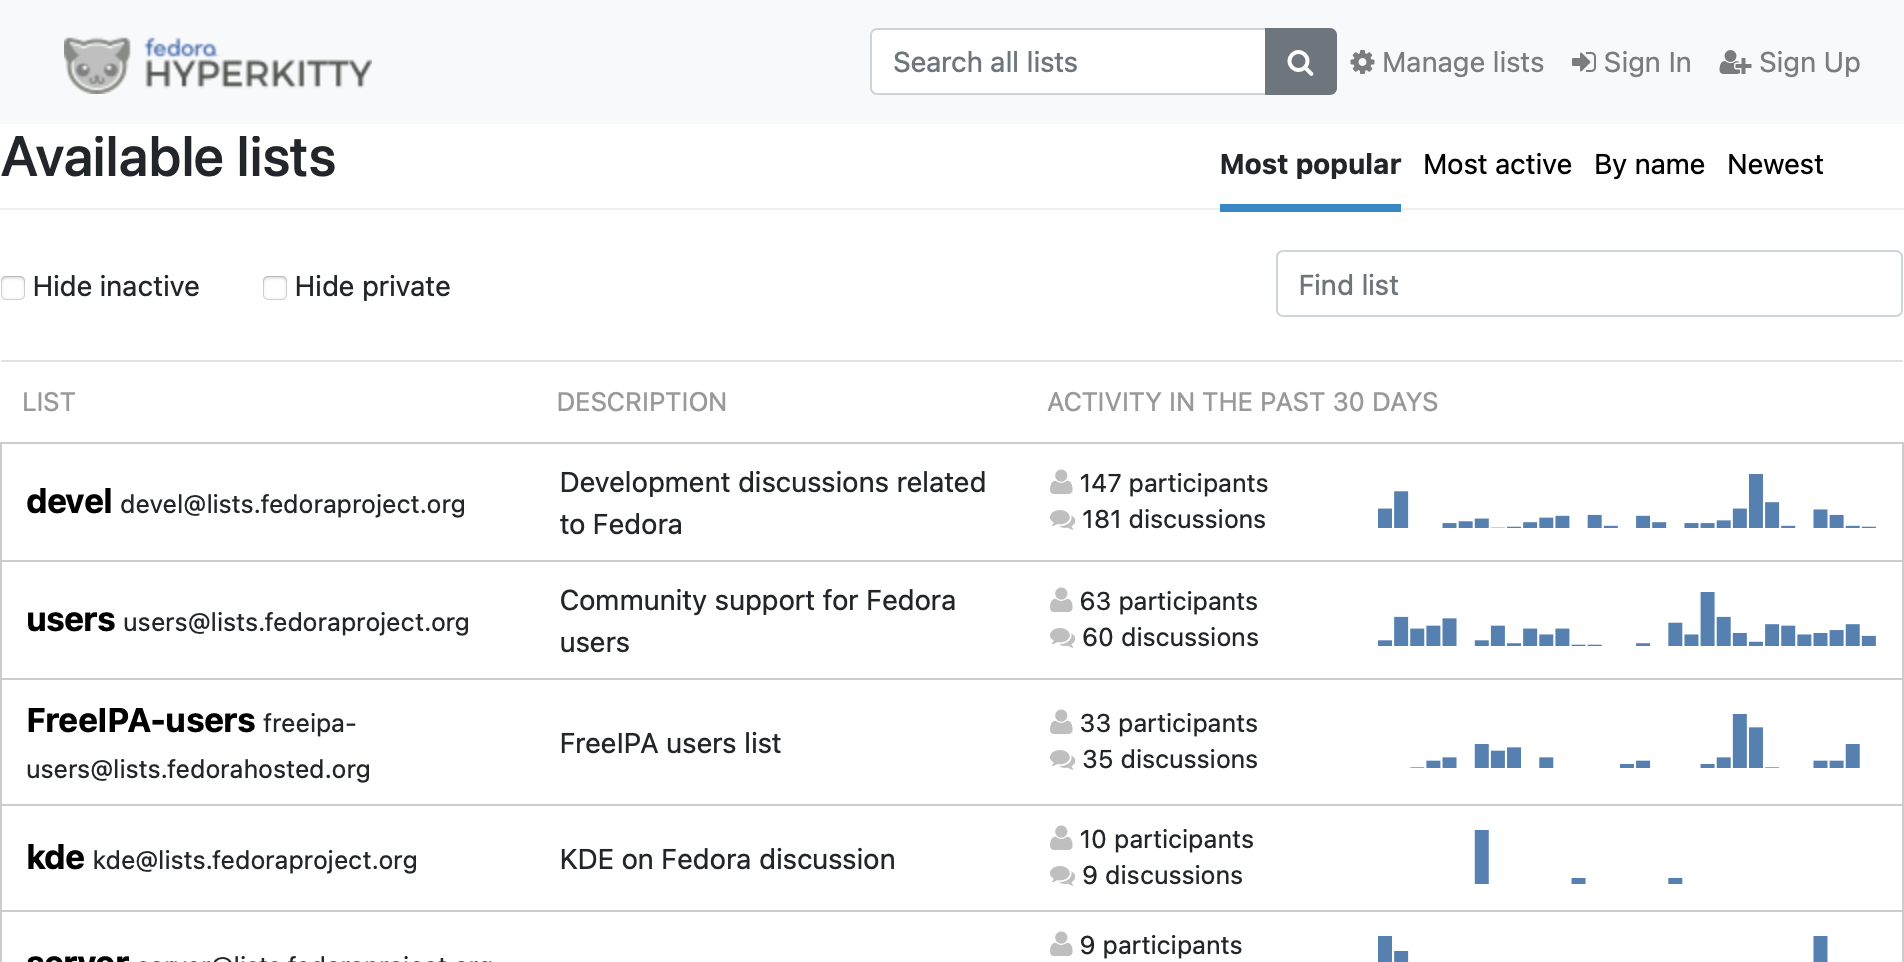
\includegraphics[width=0.9\textwidth]{imaxes/fedora-hyperkitty.png}
  \caption{Fedora Mailing lists interface}
  \label{fig:fedora-hyperkitty}
\end{figure}

While Postorius~\cite{postorius-docs} is often deployed alongside HyperKitty as part of the Mailman suite, it is not required for operation. Postorius provides a web interface for managing mailing lists, users, and settings, serving as a frontend to the REST API. However, these tasks can also be performed using the command-line tools or direct API calls.

All components of the Mailman~3 project are fully open source and licensed under the GNU General Public License (GPL), aligning with the principles of this work.

\subsection*{Sympa 7}

Sympa (version~7) is a free and open-source mailing list manager licensed under the GNU General Public License (GPL)~\cite{sympa-docs}. It is designed for scalability and flexibility, featuring a modular architecture with dedicated daemons for each task and a relational database backend. Sympa supports advanced functionality such as virtual hosting, bounce management, message archiving, and fine-grained access control.

Its web interface (WWSympa) allows users and administrators to manage subscriptions, review moderation queues, and browse archives. The software is widely used by universities and research institutions, and aligns with the principles of this work thanks to its self-hosted, open-source nature. A screenshot of the interface is shown in Figure~\ref{fig:sympa}.

\begin{figure}[H]
  \centering
  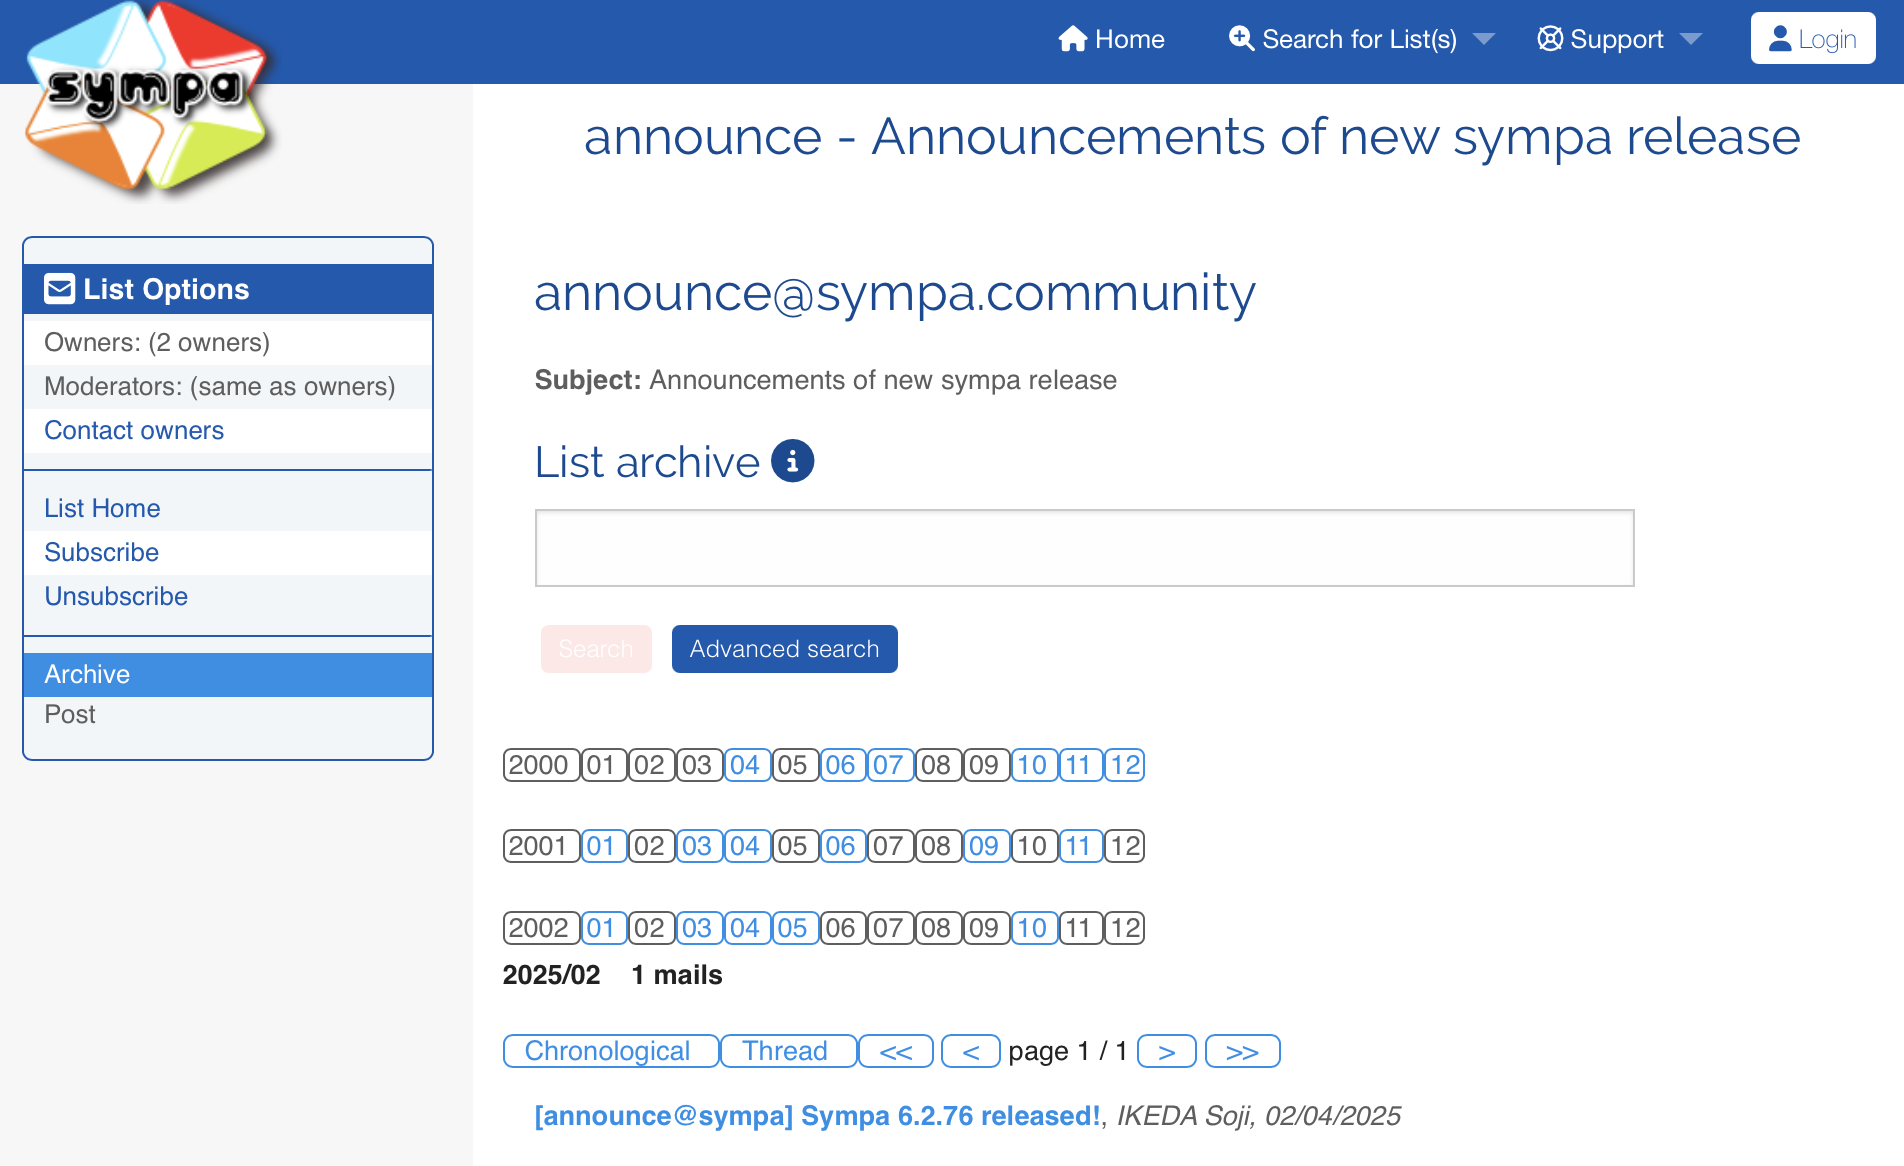
\includegraphics[width=0.9\textwidth]{imaxes/sympa.png}
  \caption{Sympa 7 interface}
  \label{fig:sympa}
\end{figure}

\subsection*{Google Groups}

Google Groups is a proprietary cloud-based mailing list and discussion service provided by Google~\cite{google-groups-docs}. It allows users to create and manage groups through a web interface, with seamless integration into the broader Google ecosystem. Due to its low administrative overhead and ease of use, it has become a widely adopted tool for informal and professional communication.

However, as a closed platform, it does not support self-hosting, customization, or full data ownership. This makes it unsuitable for privacy-conscious organizations or those with a strong preference for open-source infrastructure. Despite its limitations, Google Groups is considered in this comparison due to its mainstream adoption and minimal maintenance requirements, which may appeal to less technical communities.

%--------------------------------------------------------------------
\section{Cloud Storage / Groupware}

\textbf{Importance.} Cloud storage and groupware platforms are vital for modern organizations to manage internal documents, collaborate on projects, and streamline administrative workflows. They provide a single source of truth, ensuring data is secure and accessible to authorized members. For GPUL, this service is mission-critical as it currently hosts all administrative paperwork and invoicing. Continuity of service and granular access control are therefore essential to protect sensitive data and maintain operational stability.

\subsection*{Current stack}
\textbf{Nextcloud 24 Hub 6} deployed via Docker Compose.

\subsection*{Nextcloud Hub 10 (≈ v31)}

Nextcloud Hub 10, also known as version~31, is the latest major release of the Nextcloud platform and the direct successor to the version currently in use at GPUL. It is a self-hosted groupware solution licensed under the GNU Affero General Public License (AGPL)~\cite{nextcloud-docs}. The platform offers file storage and sharing, collaborative document editing (via OnlyOffice or Collabora), calendar and contact management, video calls, and additional features through an extensible app ecosystem.

Version~10 introduces performance improvements, including faster file uploads, optimized resource usage, and integration enhancements across components such as Files, Talk, Mail, and Calendar~\cite{nextcloud-blog}. It supports user and group management, LDAP and SSO authentication, and synchronization clients for desktop and mobile platforms. A screenshot of the interface is shown in Figure~\ref{fig:nextcloud-ui}.

\begin{figure}[H]
  \centering
  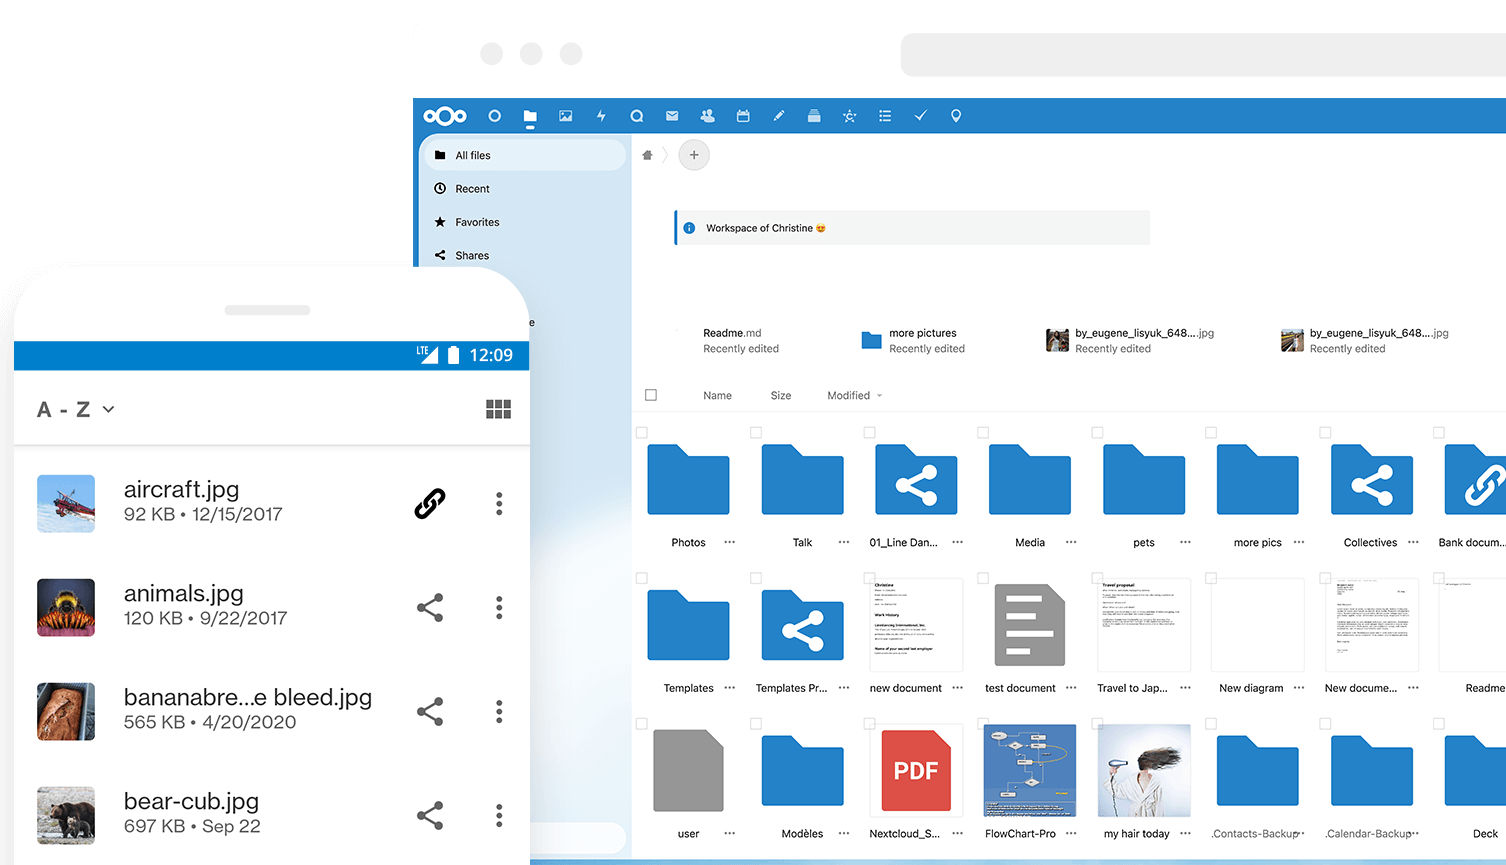
\includegraphics[width=0.9\textwidth]{imaxes/nextcloud-ui.png}
  \caption{Nextcloud Hub 10 interface}
  \label{fig:nextcloud-ui}
\end{figure}

\subsection*{ownCloud Infinite Scale}

ownCloud Infinite Scale (oCIS) is a reimplementation of the original ownCloud platform, developed as a high-performance cloud-native system written in Go~\cite{owncloud-docs}. It is licensed under the Apache License 2.0 and uses a microservices-based architecture. The system includes file synchronization and sharing, metadata management, user and role handling, and support for external storage backends~\cite{owncloud-news}.

ownCloud is the original project on which Nextcloud is based; Nextcloud was created in 2016 as a community fork of ownCloud with a separate governance and development model. oCIS introduces a redesigned backend and frontend stack, with support for container-based deployments, file firewall rules, and extended authentication options.

\subsection*{Seafile 11}

Seafile is a self-hosted file synchronization and sharing solution available under a dual license model. The Community Edition is licensed under the GNU General Public License version~3 (GPLv3), while the Professional Edition includes additional enterprise features under a commercial license~\cite{seafile-docs}. Seafile uses a content-addressable storage backend and is optimized for high performance and low latency file syncing.

Version~11 adds collaborative document editing functionality via SeaDoc, along with enhancements to its role-based access control, encryption support, and audit logging capabilities~\cite{seafile-forum}. It includes clients for desktop and mobile platforms, and supports LDAP integration.

\subsection*{Proprietary Alternatives}

Proprietary cloud storage and collaboration services such as Google Drive, Dropbox, and Microsoft 365 are widely used across various sectors. These platforms offer file sharing, document editing, and communication tools delivered as Software-as-a-Service (SaaS). They are not self-hostable and operate on third-party infrastructure, with licensing and usage conditions defined by the service providers.

%--------------------------------------------------------------------
\section{Video Conferencing Platforms}

\textbf{Importance.} Video conferencing is an indispensable tool for modern collaboration, enabling remote meetings, webinars, and virtual events. For associations, it connects geographically dispersed members and facilitates engagement with external speakers and partners. This is particularly relevant for GPUL's collaboration with external participants. A self-hosted platform would not only streamline remote coordination but also align with the association's values by ensuring data sovereignty, privacy, and a consistent, professional experience when managing meetings.

\subsection*{Current stack}

GPUL currently does not operate its own video conferencing infrastructure. Meetings are typically held using platforms chosen by external participants—most commonly Google Meet or Microsoft Teams. For internal discussions, informal coordination is sometimes done via Discord or public instances of Jitsi Meet.

\subsection*{Jitsi Meet}

Jitsi Meet is an open-source video conferencing platform licensed under the Apache 2.0 License~\cite{jitsi-docs}. It uses WebRTC and a Selective Forwarding Unit (SFU) called Jitsi Videobridge to route media between participants. An XMPP server (Prosody) handles signaling, and optional components such as Jibri enable recording and live streaming. A screenshot of the interface is shown in Figure~\ref{fig:jitsi-ui}.

\begin{figure}[H]
  \centering
  
\includegraphics[width=0.9\textwidth]{imaxes/jitsi-ui.png}
  \caption{Jitsi Cloud interface}
  \label{fig:jitsi-ui}
\end{figure}

Features include browser-based access (no registration needed), screen sharing, in-call chat, moderation tools, and integration APIs. Jitsi can be self-hosted or used via public instances such as \texttt{meet.jit.si}.

\subsection*{BigBlueButton}

BigBlueButton is a conferencing platform optimized for online learning and released under the LGPL-3.0 License~\cite{bigbluebutton-docs}. It includes tools such as whiteboards, shared notes, polling, breakout rooms, and slide presentations. Recordings can be made and replayed in a web interface. A screenshot of the interface is shown in Figure~\ref{fig:bbb-ui}.

\begin{figure}[H]
  \centering
  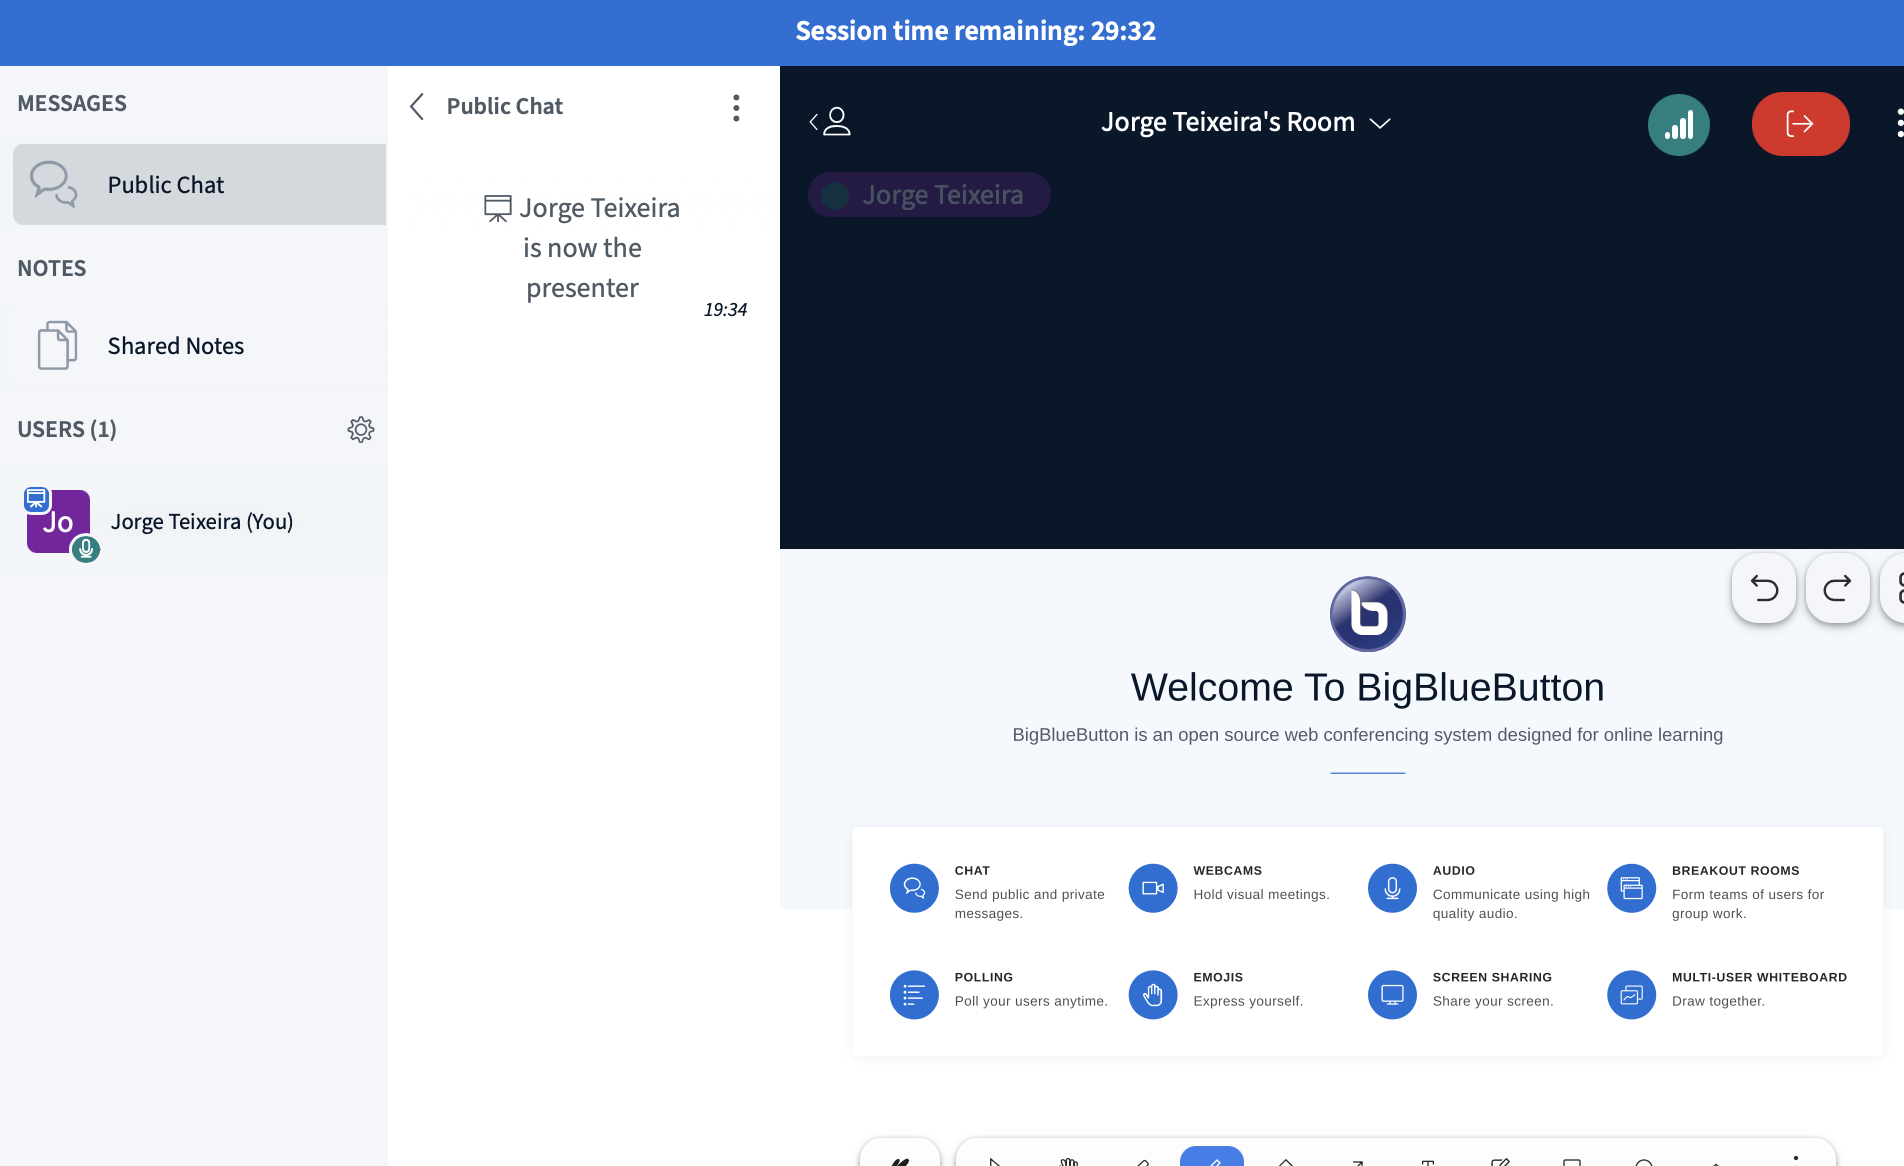
\includegraphics[width=0.9\textwidth]{imaxes/bbb-ui.png}
  \caption{BigBlueButton interface}
  \label{fig:bbb-ui}
\end{figure}

Its architecture combines WebRTC (via mediasoup), FreeSWITCH (for audio), and multiple backend services including Redis and Node.js. It requires significant system resources, making it more suitable for educational or high-capacity deployments.

\subsection*{Nextcloud Talk}

Nextcloud Talk is the communication module within the Nextcloud suite, licensed under the AGPL-3.0~\cite{nextcloud-talk-docs}. It offers one-on-one or group video calls, guest invitations, screen sharing, and chat, with end-to-end encryption.

Talk uses WebRTC for peer-to-peer connections and supports a High Performance Backend (HPB) for scalable multiparty calls via an SFU and signaling server. Integration with Nextcloud Hub 10 adds features such as calendar scheduling, file sharing, and federated chat and calls across Nextcloud instances. As GPUL already uses Nextcloud, Talk is interoperable with the existing stack.

\subsection*{Proprietary Alternatives}

Proprietary services such as Google Meet, Zoom, Microsoft Teams, and Cisco Webex are commonly used and offer feature-rich conferencing. However, they are not open-source and operate on third-party infrastructure, which raises concerns about data control and compliance. For this reason, they are not considered further in this analysis.
%--------------------------------------------------------------------
\section{Git Forges}

\textbf{Importance.} A Git forge is a collaborative hub for software development, providing essential tools like issue tracking, pull requests, and CI/CD. For community-driven projects, a user-friendly forge is crucial for lowering the barrier to entry and streamlining contributor workflows. While not every association develops software, it is a key activity for GPUL. A modern forge is therefore essential to ease contributor onboarding and consolidate development, moving beyond the limitations of a legacy \texttt{git daemon}.

\subsection*{Current stack}
The current setup combines a legacy \verb|git daemon| exposed over SSH and HTTP with GitHub repositories. Most active development and contribution workflows have migrated to GitHub, while the \texttt{git daemon} continues to serve older repositories.

\subsection*{Gitea 1.23 and Forgejo}

Gitea is an open-source Git forge licensed under the MIT license~\cite{gitea-docs}, designed for self-hosted deployment. It provides Git repository hosting with features such as issue tracking, pull requests, project wikis, Kanban boards, and integrated \gls{cicd} via Gitea Actions. Forgejo is a community-driven fork of Gitea initiated in 2022, also under the MIT license~\cite{forgejo-docs}. Both platforms share the same core functionality and user experience.

A screenshot of the Gitea interface is shown in Figure~\ref{fig:gitea-ui}.

\begin{figure}[H]
  \centering
  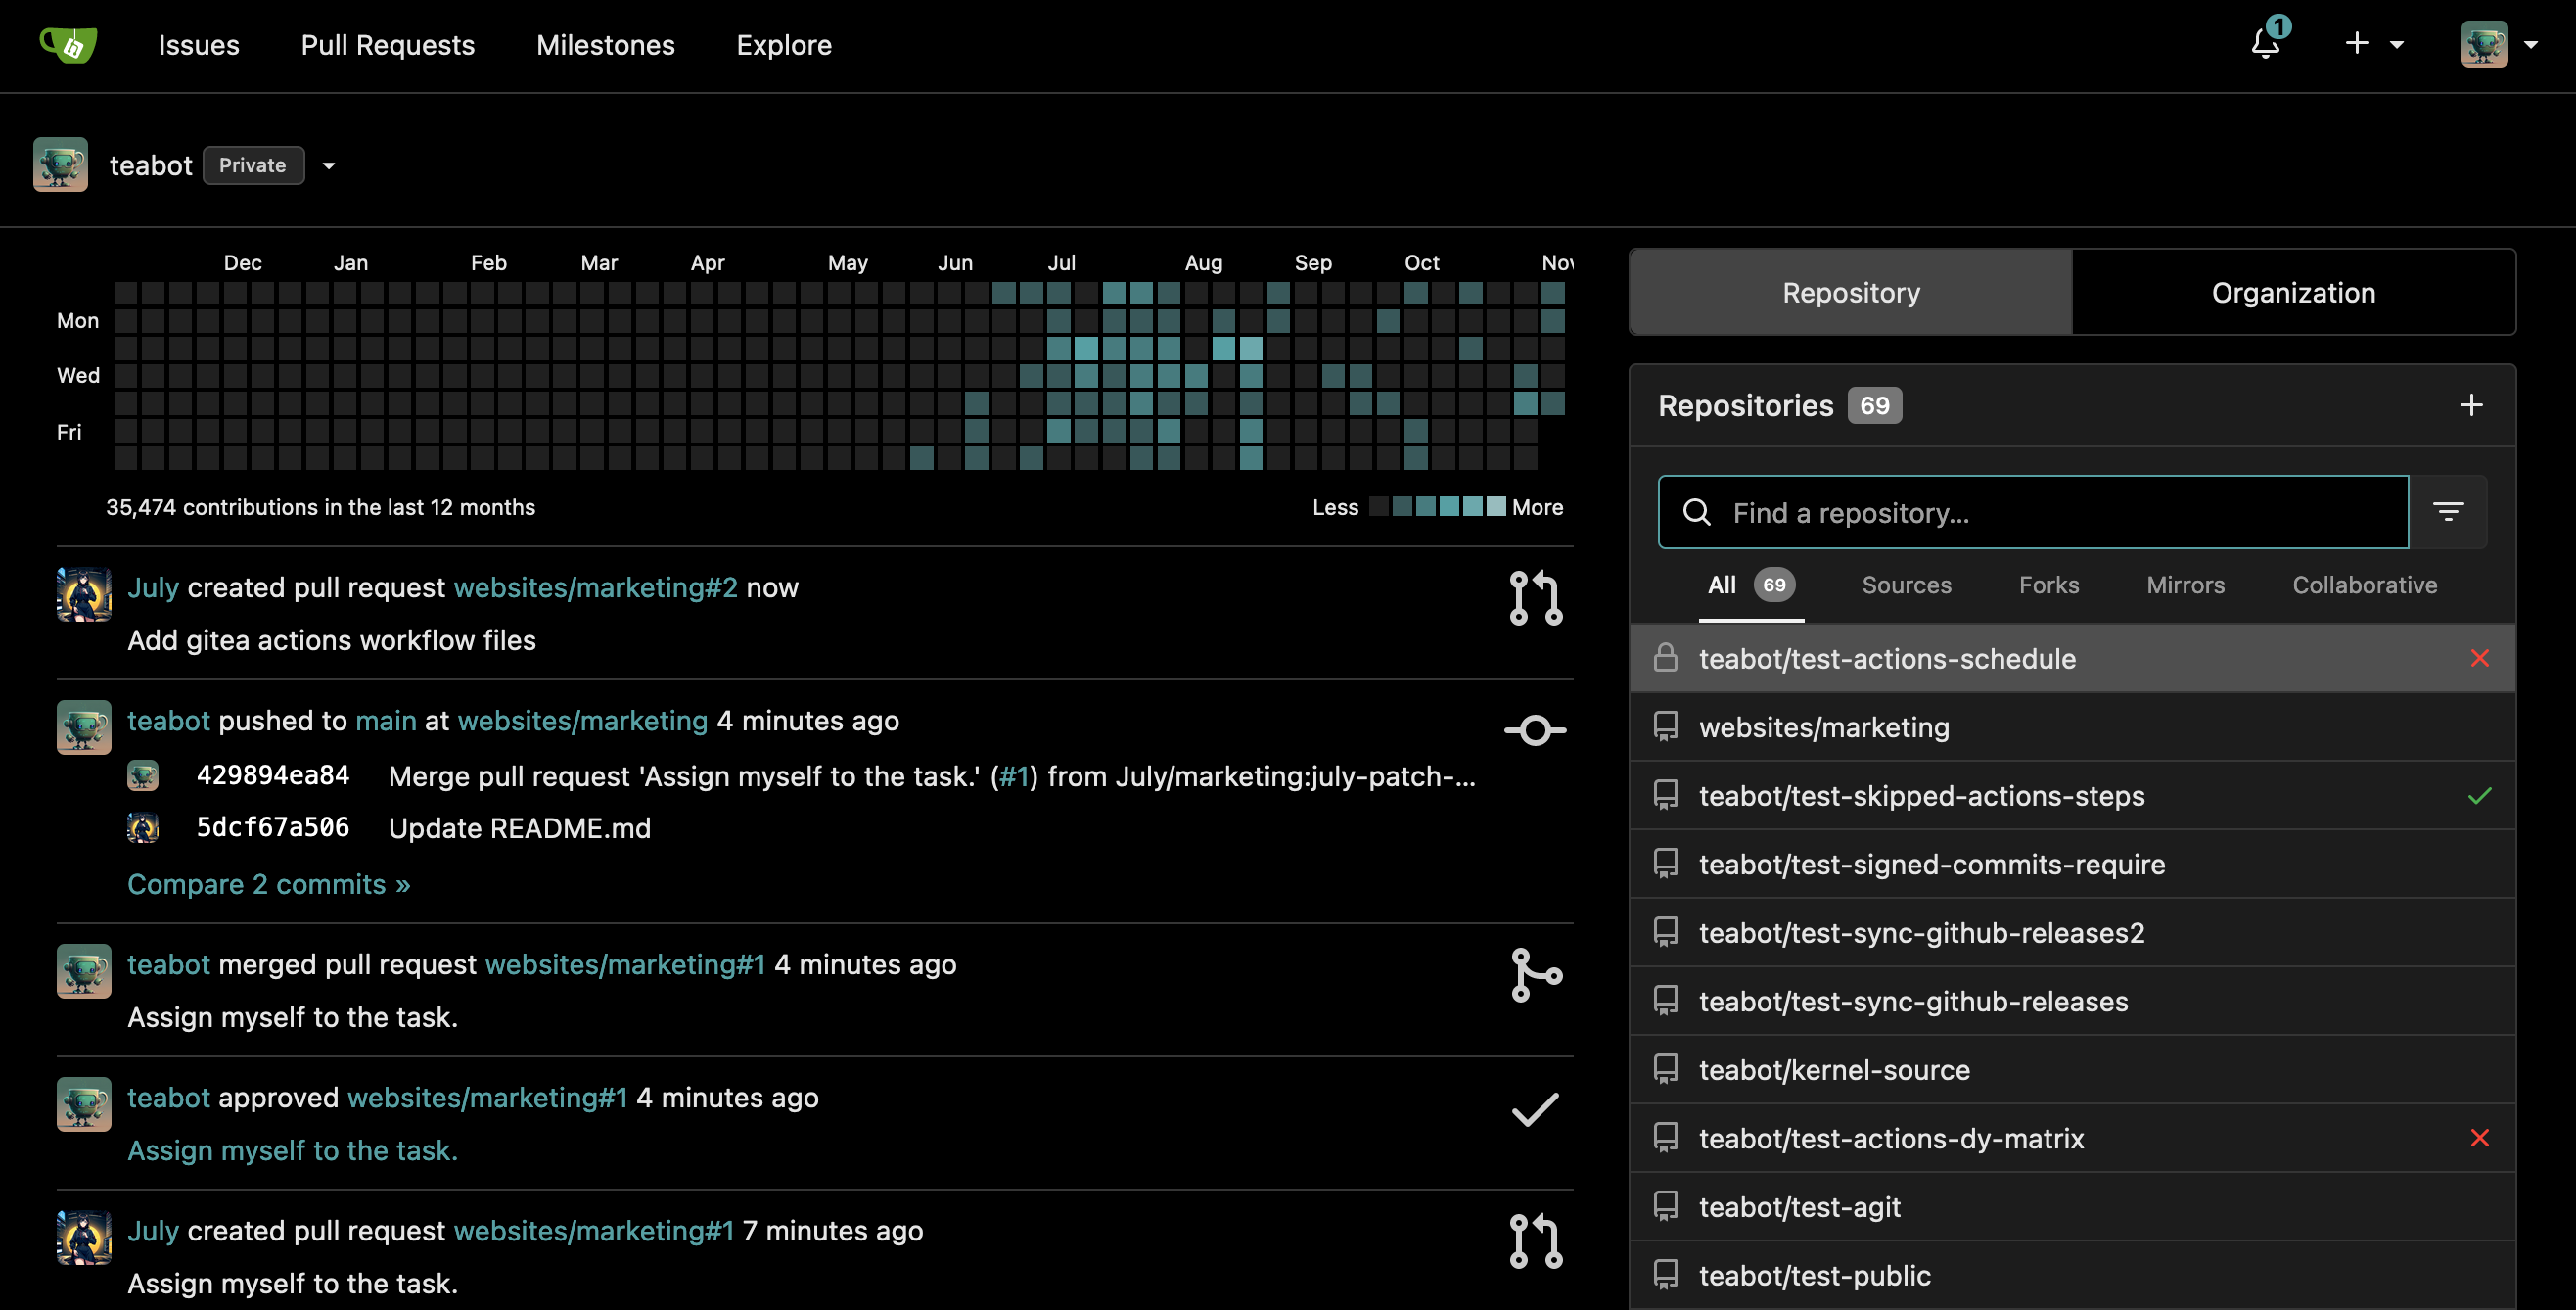
\includegraphics[width=0.9\textwidth]{imaxes/gitea-ui.png}
  \caption{Gitea interface}
  \label{fig:gitea-ui}
\end{figure}

\subsection*{GitLab CE 18.0}

GitLab Community Edition (CE) is an open-source Git forge licensed under the MIT license~\cite{gitlab-docs}. It supports both self-hosted and cloud-hosted deployment. GitLab CE provides Git repository management, issue tracking, merge requests, wikis, and a native \gls{cicd} system. Additional tools include container registry support, role-based access control, and project analytics.

\subsection*{GitHub}

GitHub is a proprietary Git forge provided as a cloud-based service~\cite{github-docs}. It includes Git repository hosting, pull requests, issue tracking, integrated GitHub Actions for \gls{cicd}, project boards, and repository wikis. While a self-hosted variant exists (GitHub Enterprise), most users interact through GitHub.com.

GPUL currently uses GitHub alongside a legacy \texttt{git daemon}. A screenshot of the GitHub interface is shown in Figure~\ref{fig:github-ui}.

\begin{figure}[H]
  \centering
  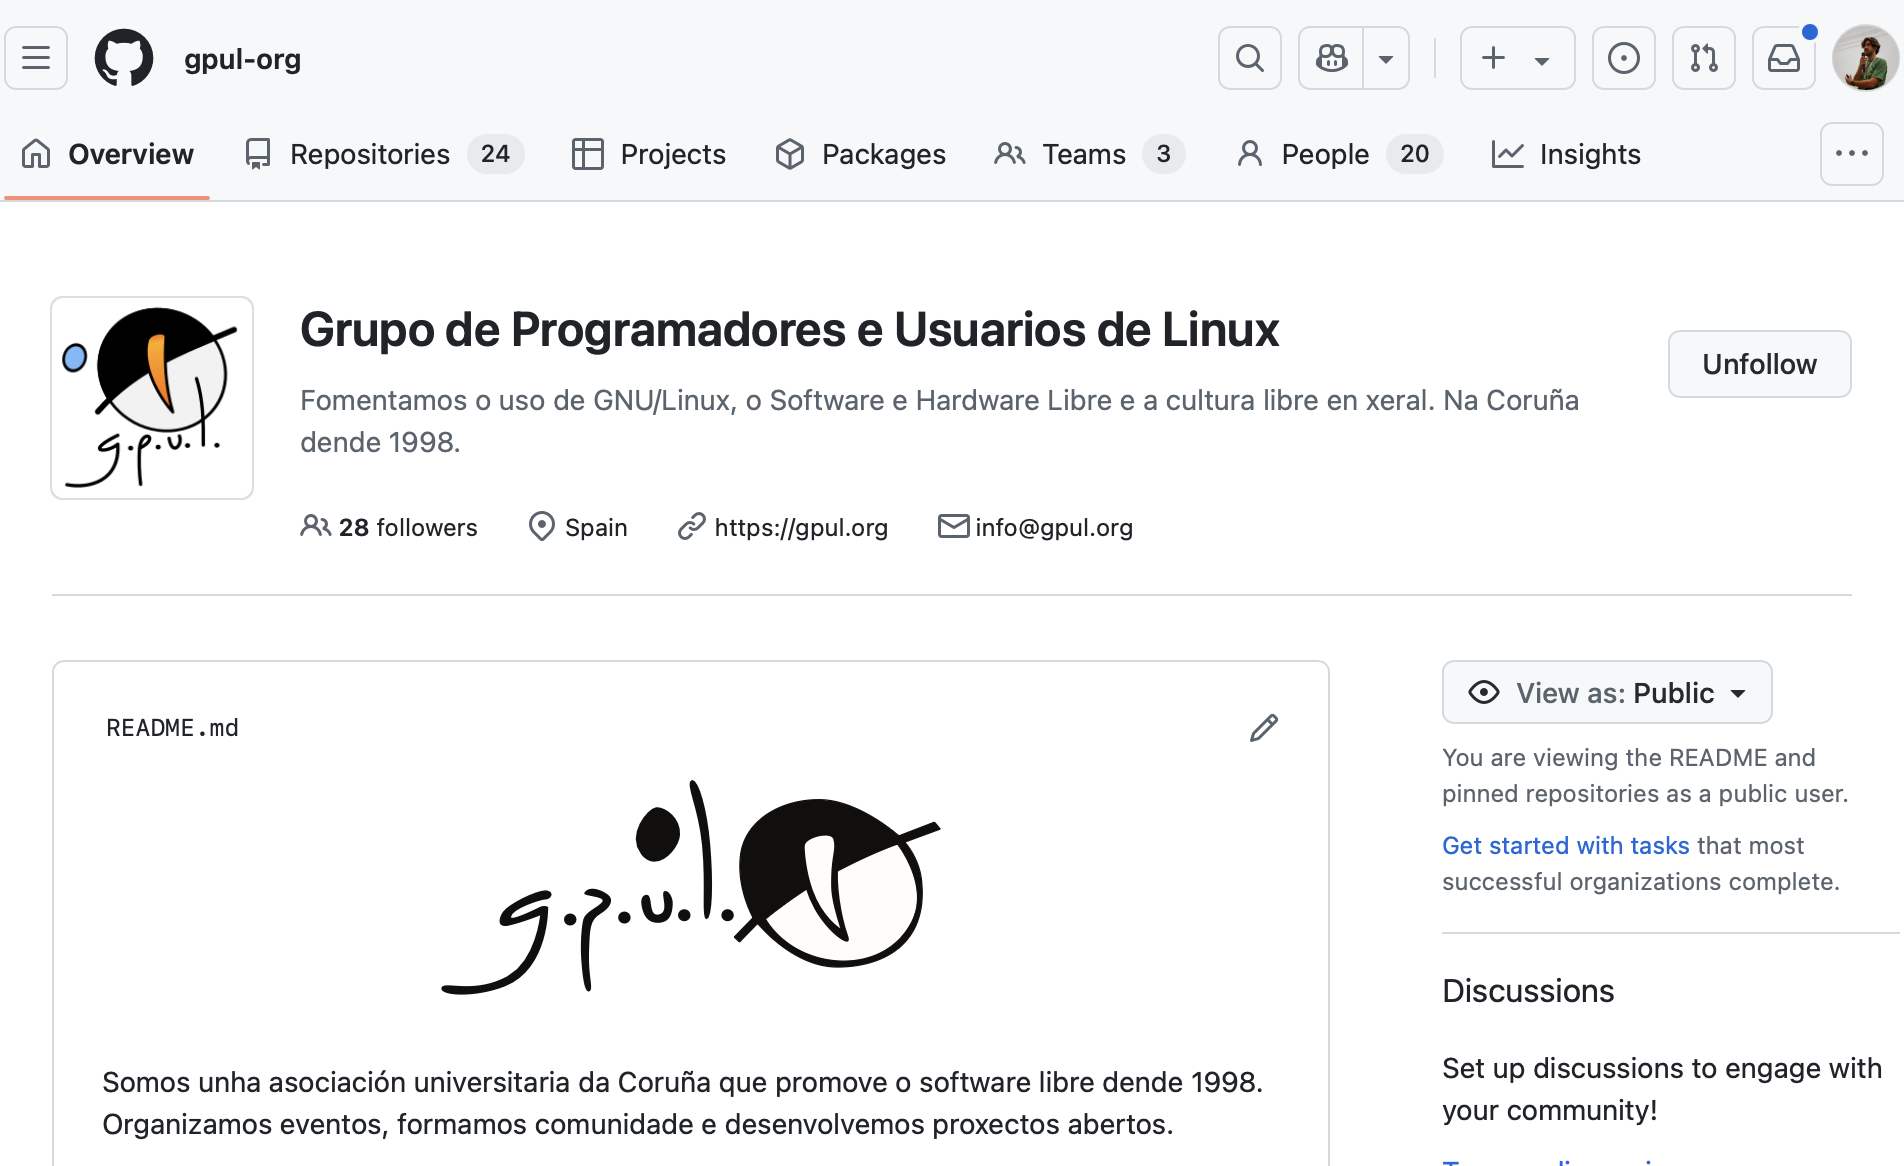
\includegraphics[width=0.9\textwidth]{imaxes/github-ui.png}
  \caption{GitHub organization interface}
  \label{fig:github-ui}
\end{figure}

%--------------------------------------------------------------------
\section{Team Chat Platforms}

\textbf{Importance.} Real-time chat platforms are the central hub for informal communication and day-to-day coordination in many organizations. They foster community engagement, enable rapid problem-solving, and are invaluable for onboarding new members. For a community-driven association like GPUL, such a platform is essential for both synchronous and asynchronous interactions. Adopting a self-hosted solution would also provide full data ownership and control over the primary communication tool, aligning with the association's core values.

\subsection*{Current stack}

GPUL currently uses a mix of Telegram and Discord for day-to-day communication. While both are widely adopted and convenient, they are externally managed proprietary platforms. This limits flexibility, ownership, and long-term sustainability of the communication infrastructure.

\subsection*{Matrix (Element)}

Matrix is an open standard protocol for real-time communication, supporting decentralization and end-to-end encryption. It operates through independently hosted \emph{homeservers}, which synchronize using federation. The most widely used homeserver implementation is \texttt{Synapse}, written in Python. The reference client, \texttt{Element}, provides a web-based interface with features such as threads, rooms, voice/video calls, and file sharing. Federation and bridging to other platforms (e.g., IRC, Slack, Discord) are natively supported. Matrix is licensed under the Apache License 2.0~\cite{matrix-docs}. A screenshot of the Element interface is shown in Figure~\ref{fig:element-ui}.

\begin{figure}[H]
  \centering
  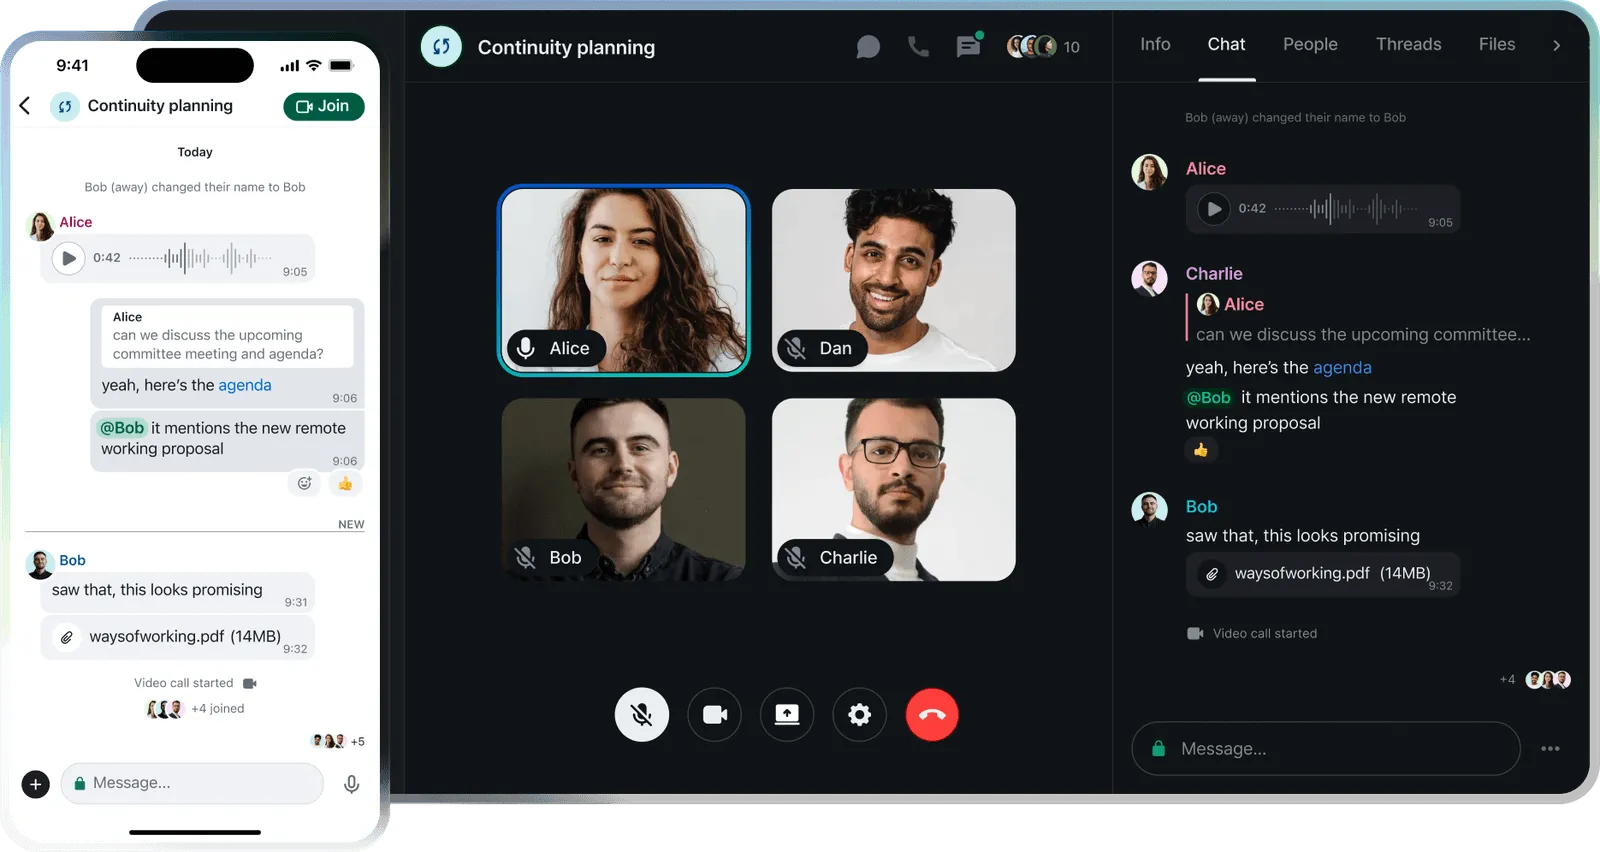
\includegraphics[width=0.9\textwidth]{imaxes/element-ui.png}
  \caption{Element interface}
  \label{fig:element-ui}
\end{figure}

\subsection*{Mattermost}

Mattermost is a self-hosted team messaging platform released under the MIT License~\cite{mattermost-docs}. It provides channel-based discussions, searchable history, file attachments, and integrations through slash commands, bots, and plugins. The architecture is monolithic and typically deployed with a PostgreSQL backend. Mattermost supports SSO, LDAP, and OAuth2 authentication, and offers a web interface, desktop, and mobile clients. A screenshot of the Mattermost interface is shown in Figure~\ref{fig:mattermost-ui}.

\begin{figure}[H]
  \centering
  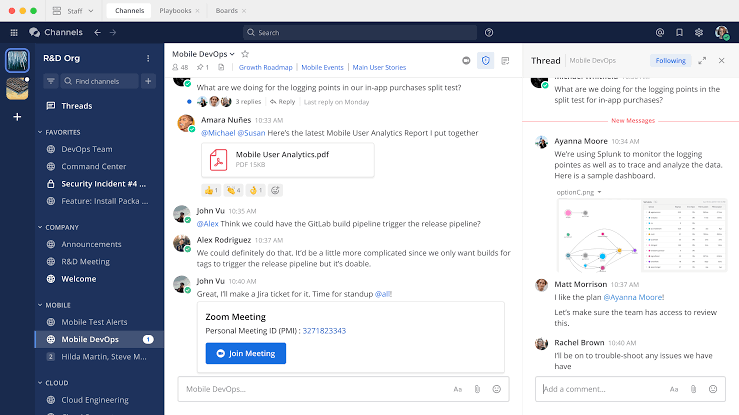
\includegraphics[width=0.9\textwidth]{imaxes/mattermost-ui.png}
  \caption{Mattermost interface}
  \label{fig:mattermost-ui}
\end{figure}

\subsection*{Nextcloud Talk (Chat)}

Nextcloud Talk includes a chat component within the broader Nextcloud groupware ecosystem. It allows persistent one-to-one and group conversations with notifications and shared file integration. The code is licensed under AGPLv3~\cite{nextcloud-talk-docs}.

\subsection*{Proprietary Alternatives}

Closed-source platforms like Discord, Slack, and Telegram offer feature-rich environments but rely on external servers and proprietary ecosystems. These tools are not further considered due to the lack of data sovereignty and alignment with the association's open-source values.

%--------------------------------------------------------------------
\section{Secrets / Password Vault}

\textbf{Importance.} Securely managing shared credentials is a fundamental security requirement for any organization. Password vaults provide encrypted storage, role-based access control, and auditability, mitigating the significant risks associated with ad-hoc methods like sharing plaintext files. This is a critical need for GPUL, whose current practices are insecure. Implementing a dedicated vault is essential to protect the association's infrastructure, services, and member data.

\subsection*{Current stack}
GPUL currently stores shared passwords in a plaintext file within the Nextcloud instance. This solution lacks encryption, granular access control, and audit trails.

\subsection*{Bitwarden Server}
Bitwarden is a password manager licensed under AGPLv3 with both a self-hosted server and an official cloud offering. It supports client-side AES-256 encryption, role-based access control, and sharing via collections and groups. Vaults are stored in a PostgreSQL database with encrypted attachments. Comprehensive documentation is available online~\cite{bitwarden-docs}.

\begin{figure}[H]
  \centering
  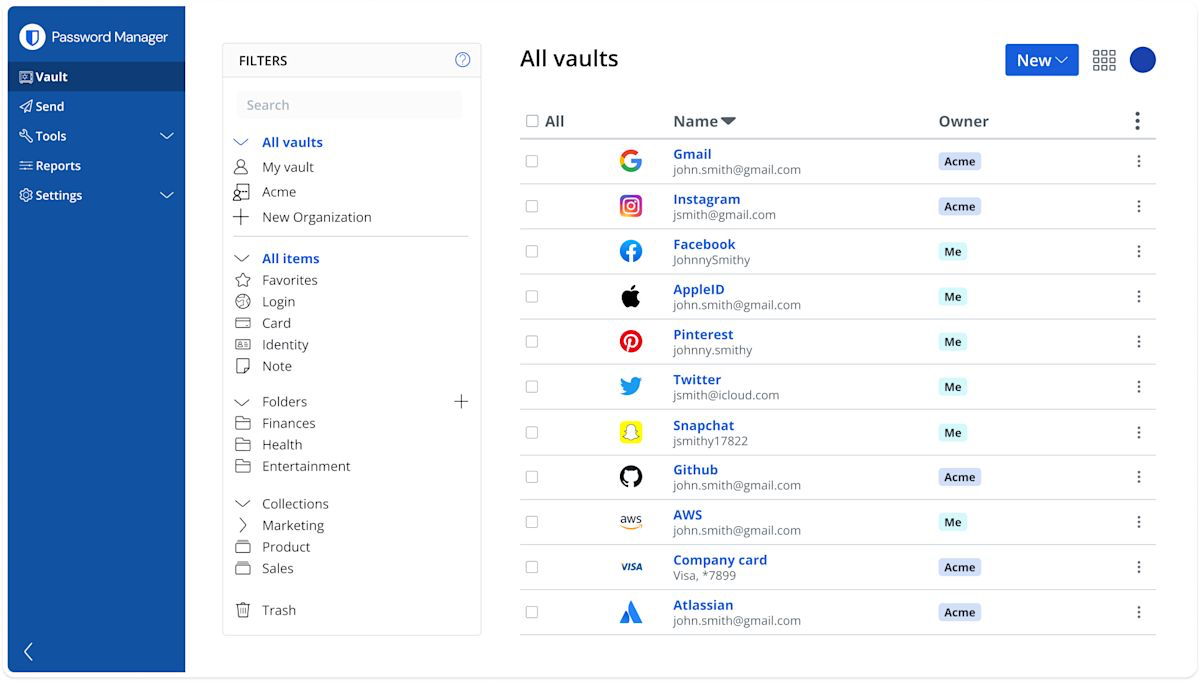
\includegraphics[width=0.9\textwidth]{imaxes/bitwarden-ui.png}
  \caption{Bitwarden interface}
  \label{fig:bitwarden-ui}
\end{figure}

\subsection*{Passbolt 4}
Passbolt is a web-based team password manager licensed under AGPLv3~\cite{passbolt-security}. It uses OpenPGP encryption in the browser, with each password encrypted for specific users' keys. It supports fine-grained sharing, activity logs, and role-based access, and uses a MySQL-compatible backend. Unlike Bitwarden, it requires users to manage their private GPG keys. A screenshot of the interface is shown in Figure~\ref{fig:passbolt-ui}.

\begin{figure}[H]
  \centering
  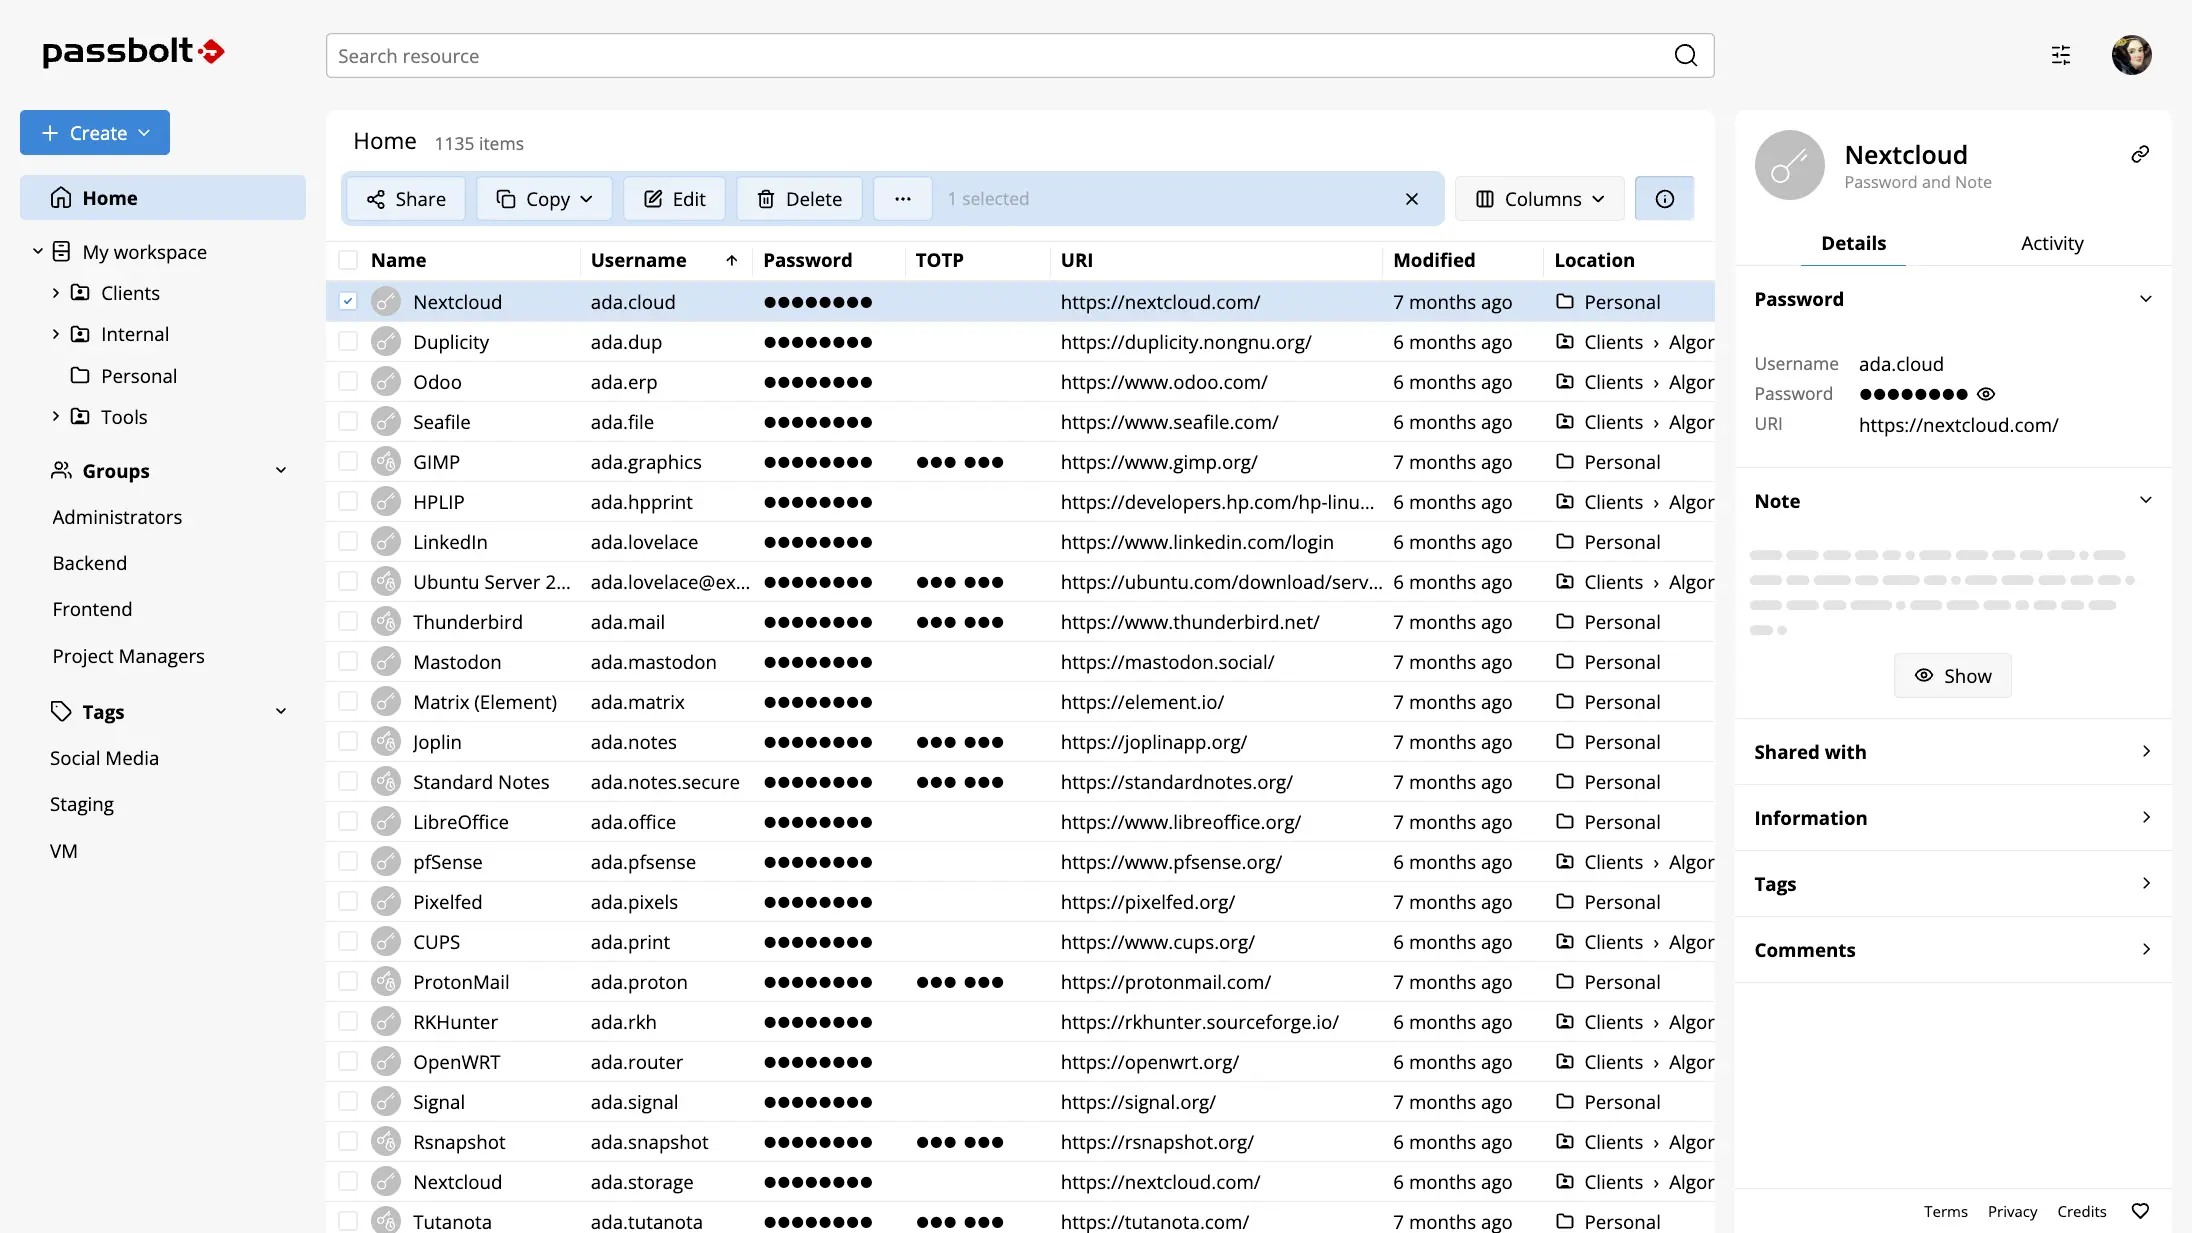
\includegraphics[width=0.9\textwidth]{imaxes/passbolt-ui.png}
  \caption{Passbolt interface}
  \label{fig:passbolt-ui}
\end{figure}

\subsection*{HashiCorp Vault 1.17}
Vault is a general-purpose secrets manager aimed at infrastructure-level secrets rather than password sharing. It supports dynamic secrets, time-to-live (TTL) credentials, and multiple authentication backends (e.g., GitHub, LDAP). Secrets are encrypted server-side and stored in a pluggable backend such as files, Consul, or PostgreSQL. Vault is source-available under the BSL 1.1 license~\cite{vault-bsl}.

\subsection*{Proprietary Alternatives}
Popular proprietary services like 1Password, LastPass, and Keeper offer similar functionality but require the use of externally hosted infrastructure. Due to GPUL's preference for open-source and self-hosted tools, these are excluded from further evaluation.

%--------------------------------------------------------------------
\section{Monitoring \& Logging}

\textbf{Importance.} Monitoring and logging are essential for ensuring the stability and performance of critical services, providing visibility into system behavior to help administrators detect and resolve issues proactively. For a volunteer-run, community-managed infrastructure like GPUL's, where resources are limited and continuity is key, a reliable observability setup is not a luxury but a necessity. It is crucial for preventing service degradation, reducing downtime, and easing the burden on future maintainers.

\subsection*{Current stack}
Currently, no formal monitoring stack is in place. Most services log to local files with no rotation configured, often resulting in uncontrolled disk usage. There is no log centralization, alerting, or metric tracking, making it difficult to respond proactively to incidents.

\subsection*{Prometheus + Grafana + Loki}
A popular open source stack for monitoring and logging is the combination of Prometheus, Grafana, and Loki. Prometheus is a time-series database and alerting system that collects numeric metrics from instrumented services via HTTP endpoints~\cite{prometheus-docs}. It supports service discovery, pull-based scraping, and label-based queries using PromQL. Grafana acts as a dashboard and visualization layer, connecting to Prometheus and other sources to present interactive panels, graphs, and alerts. Loki is a log aggregation system inspired by Prometheus: it stores log streams with associated labels, allowing queries using LogQL~\cite{loki-docs}. Unlike traditional log engines, Loki only indexes metadata, making it efficient and lightweight. A screenshot of the Grafana interface is shown in Figure~\ref{fig:grafana-ui}.

\begin{figure}[H]
  \centering
  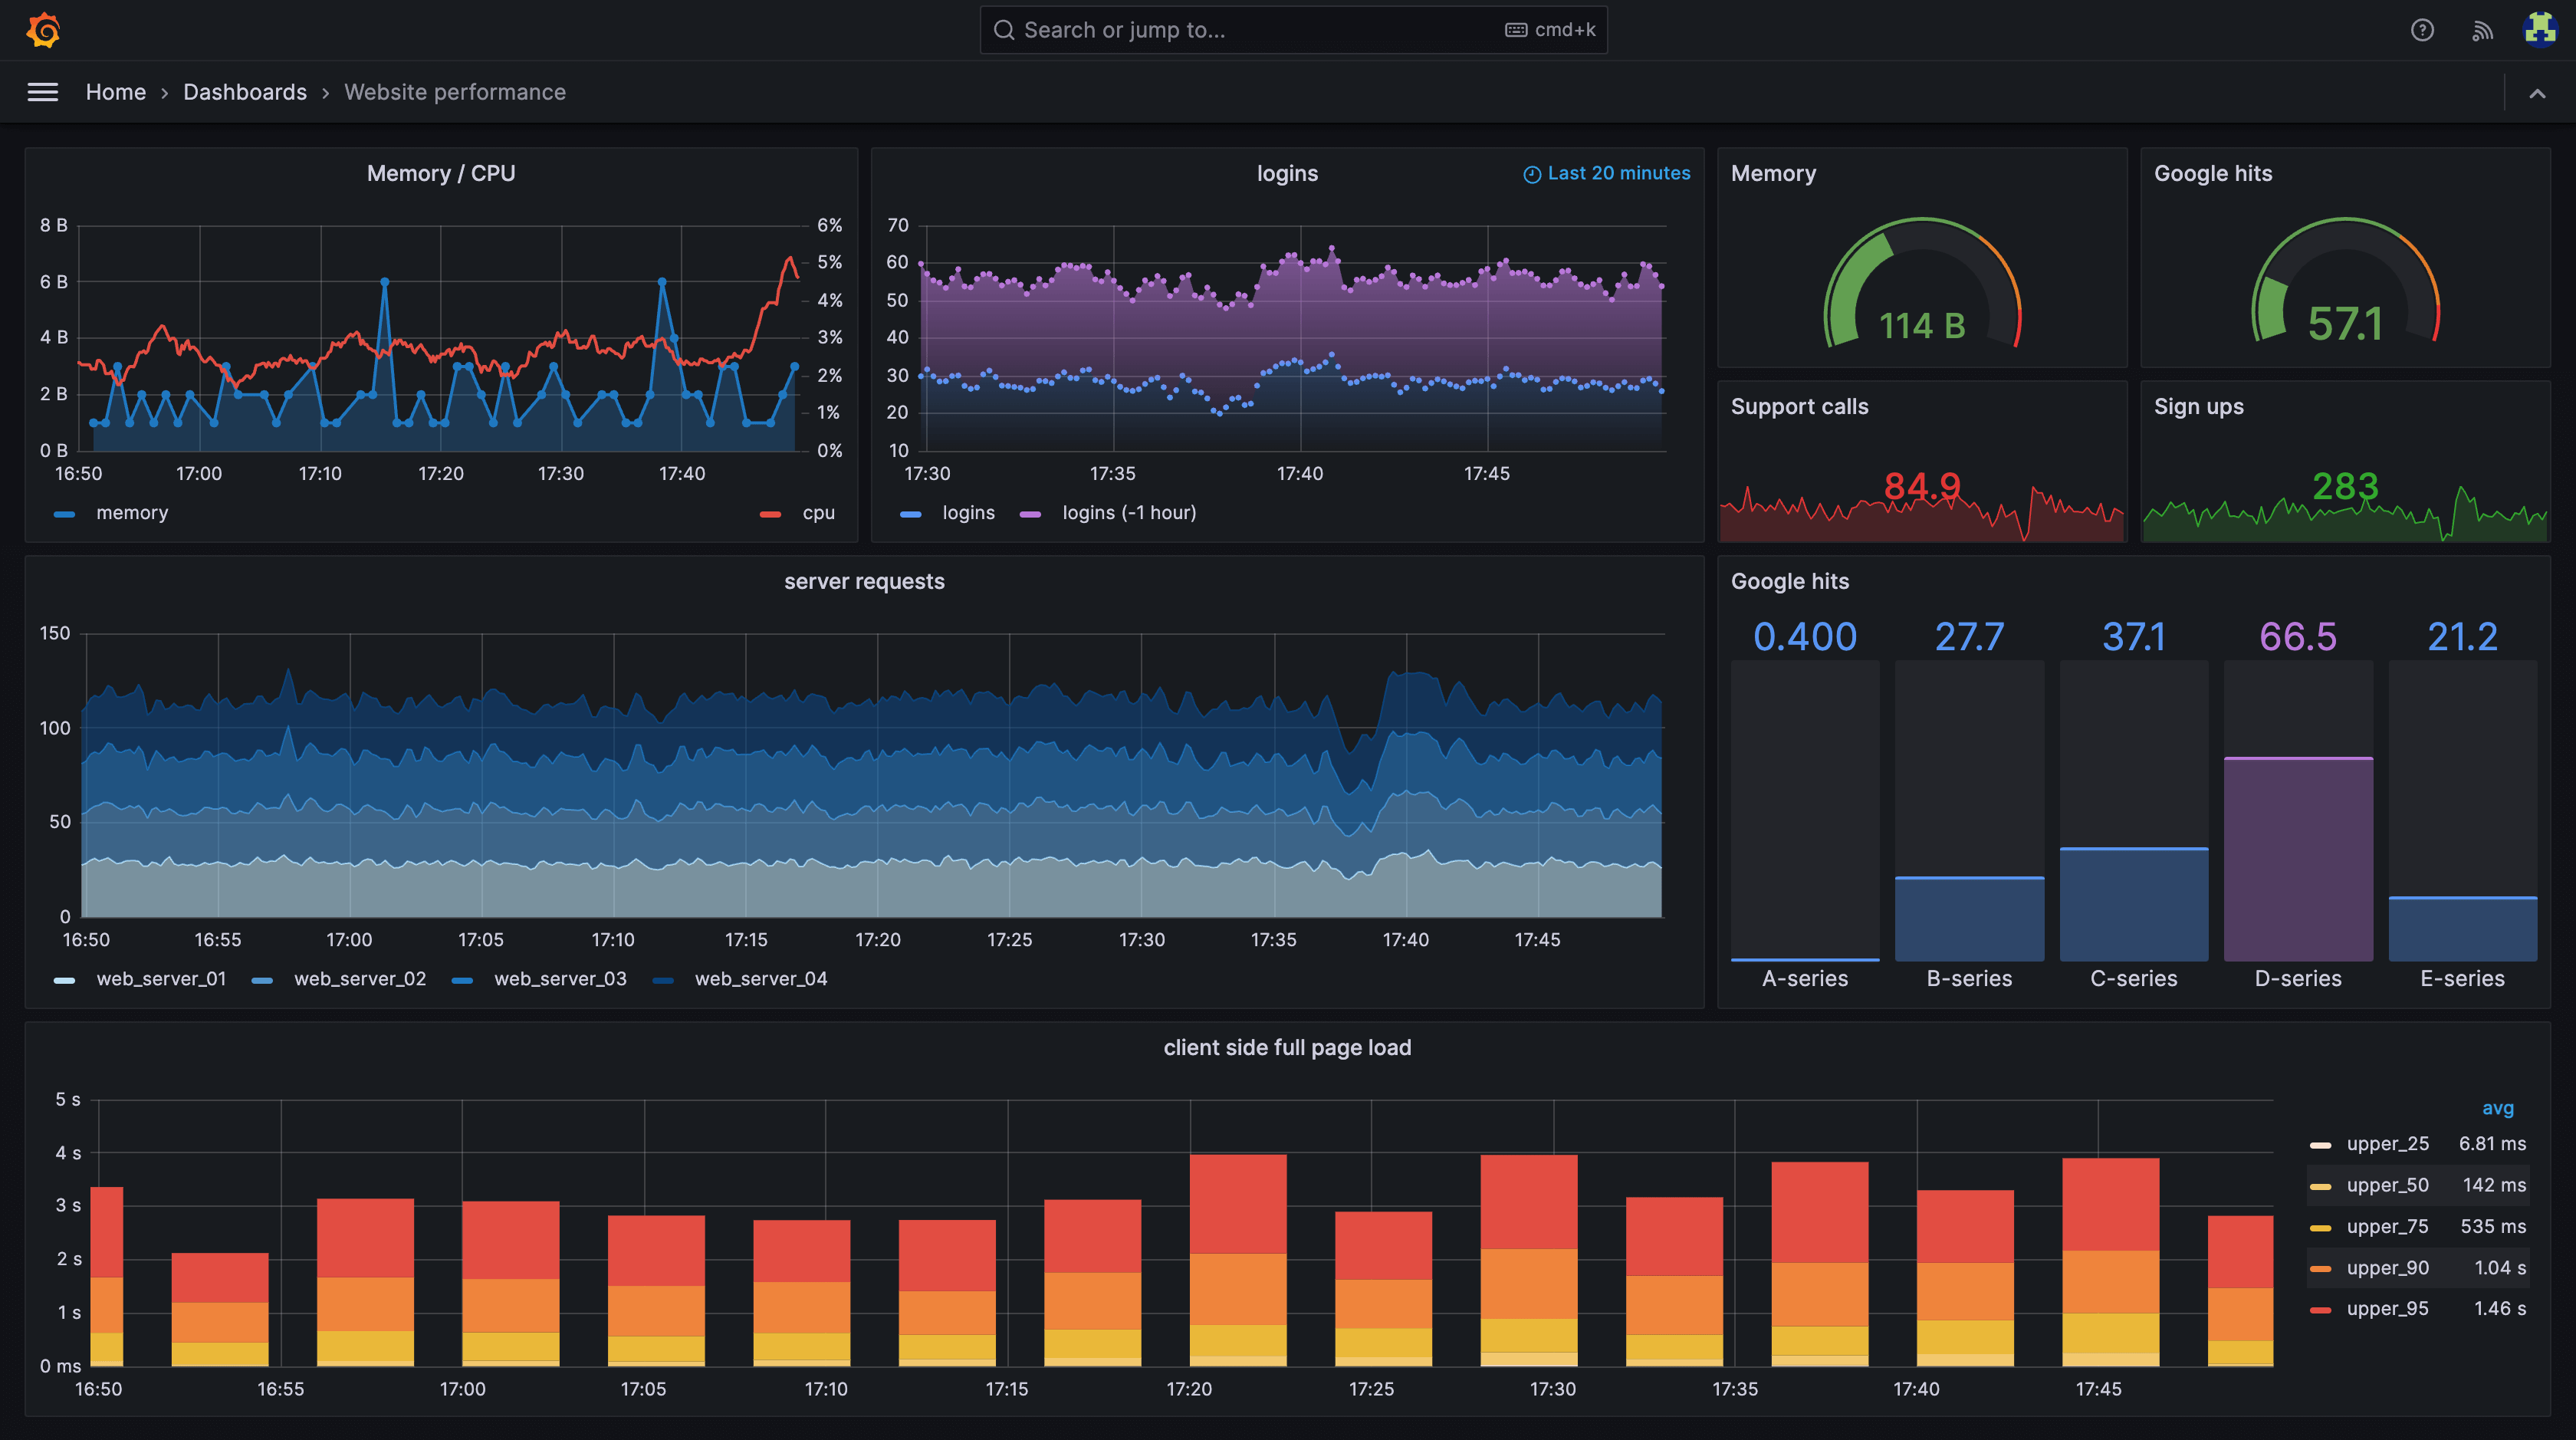
\includegraphics[width=0.9\textwidth]{imaxes/grafana-ui.png}
  \caption{Grafana interface}
  \label{fig:grafana-ui}
\end{figure}

Each component is open source: Prometheus is under the Apache 2.0 license, while Grafana and Loki are licensed under AGPLv3~\cite{grafana-license-change}. Together, they form a well-integrated observability suite, often referred to as the PLG stack.

\subsection*{Zabbix}
Zabbix is a mature open source monitoring solution that uses a central server and lightweight agents~\cite{zabbix-web}. It supports metric collection through agents, SNMP, IPMI, and scriptable checks. Zabbix provides a web interface for dashboards and alerts, and includes automatic discovery, distributed proxies, and a large template library. It stores metrics in SQL databases and is licensed under AGPLv3. A screenshot of the interface is shown in Figure~\ref{fig:zabbix-ui}.

\begin{figure}[H]
  \centering
  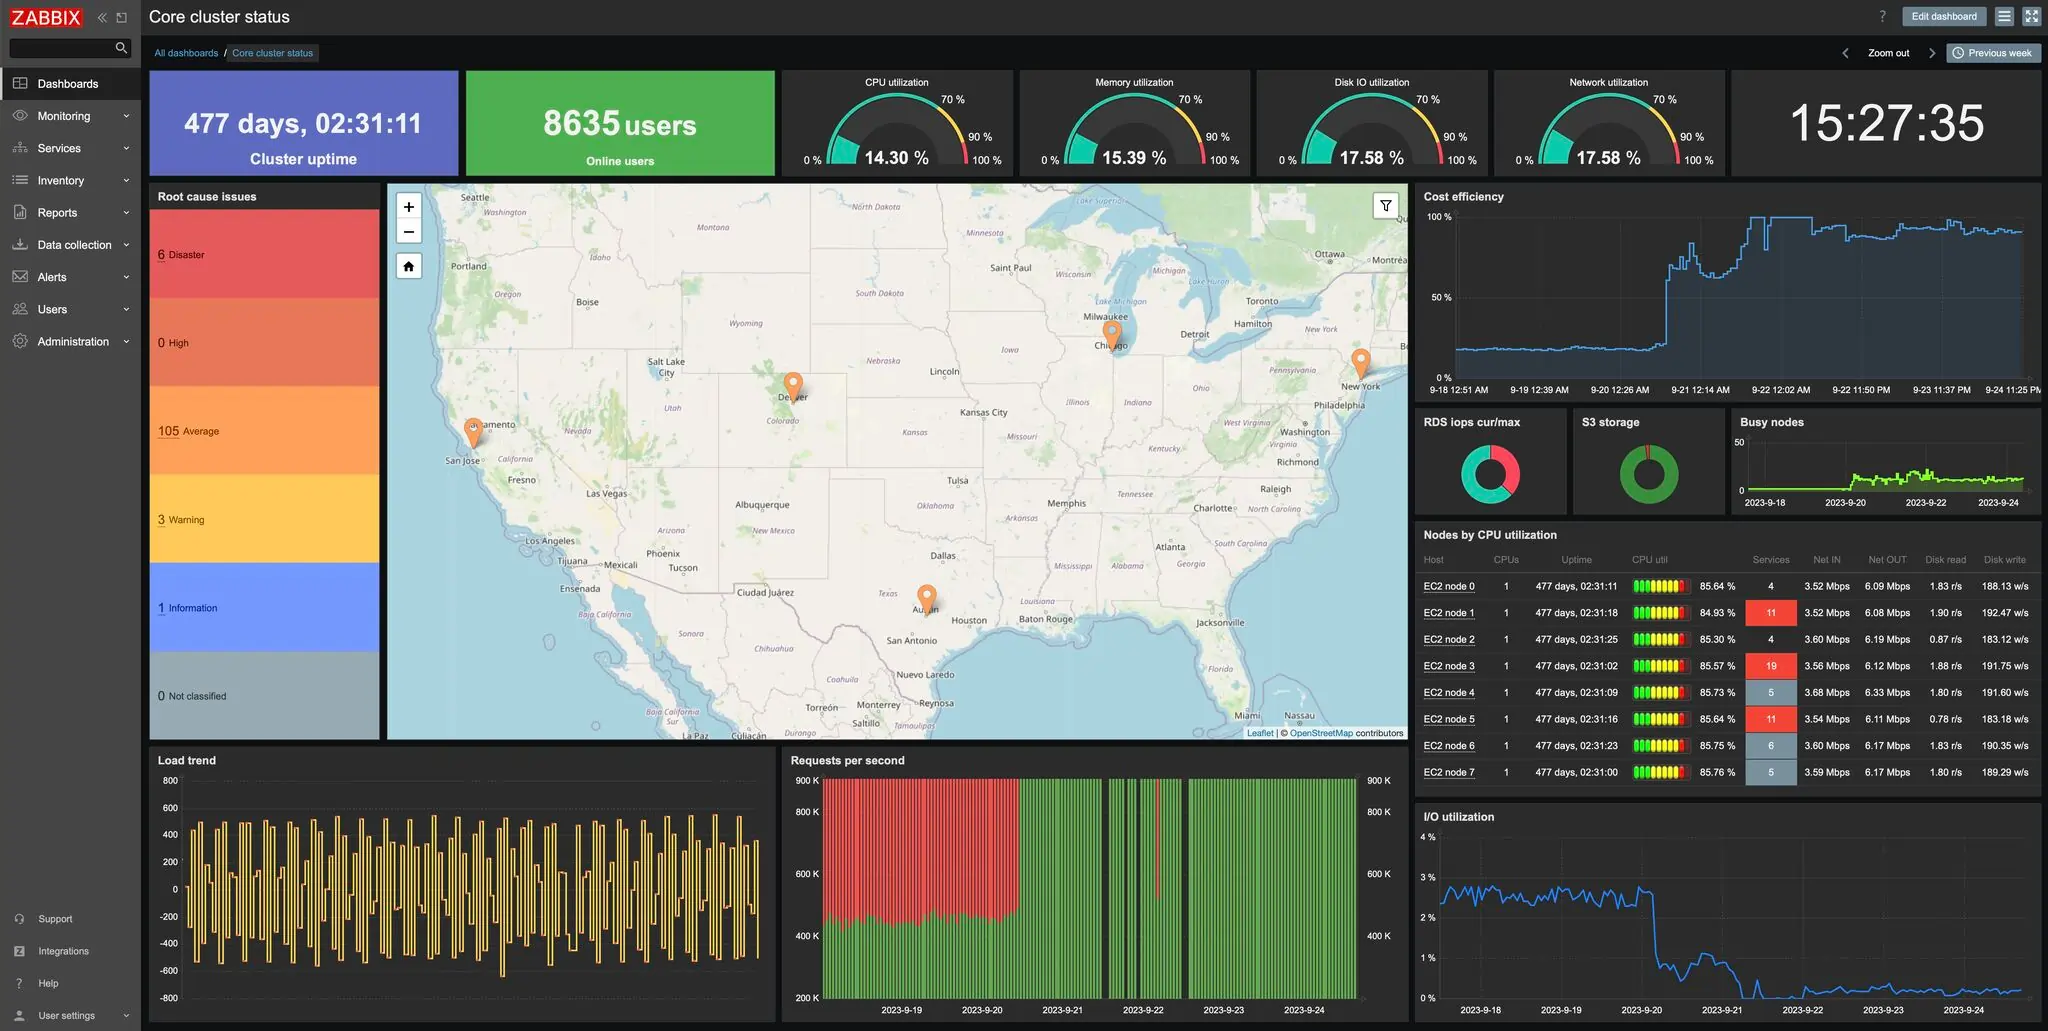
\includegraphics[width=0.9\textwidth]{imaxes/zabbix-ui.png}
  \caption{Zabbix interface}
  \label{fig:zabbix-ui}
\end{figure}

\subsection*{OpenSearch Dashboards (formerly ELK)}
The ELK stack—Elasticsearch, Logstash, and Kibana—is widely used for log aggregation and analysis. Elasticsearch handles indexing and querying, Logstash parses and ships logs, and Kibana provides visualization. The original ELK stack shifted away from open source licenses, but forks like OpenSearch continue under Apache 2.0~\cite{opensearch-web}. Alternatively, Elastic recently reintroduced AGPLv3 licensing for their stack~\cite{elastic-license}. While powerful, the ELK/OpenSearch stack is resource-intensive and typically more complex to manage.

\subsection*{Proprietary Alternatives}
Cloud-based observability platforms such as Datadog, New Relic, and Splunk offer complete solutions with minimal setup and powerful features. However, their pricing models, data sovereignty implications, and closed-source nature make them less suitable for GPUL's goals of open, self-hosted, and cost-effective infrastructure~\cite{datadog-web}.

%--------------------------------------------------------------------
\section{Event Ticketing \& CFP Tooling}

\textbf{Importance.} For many associations, events are a core activity requiring tools for ticketing, registration, and speaker management. An integrated platform can streamline these workflows, reduce administrative overhead, and improve the experience for organizers and attendees. Events are a fundamental part of GPUL's community outreach, but the current reliance on separate proprietary services introduces friction and cost. Adopting a unified, self-hosted tool would align with the association's values while providing greater control and a more professional appearance.

\subsection*{Current stack}
GPUL currently uses a mix of proprietary platforms. \emph{Meetup} is used to promote and coordinate free, recurring meetups. For larger events requiring registration and payment, \emph{Eventbrite} is employed. For call-for-proposals (CFPs), the hosted service \emph{pretalx.com} has been used. A screenshot of the Meetup interface is shown in Figure~\ref{fig:meetup-ui}.

\begin{figure}[H]
  \centering
  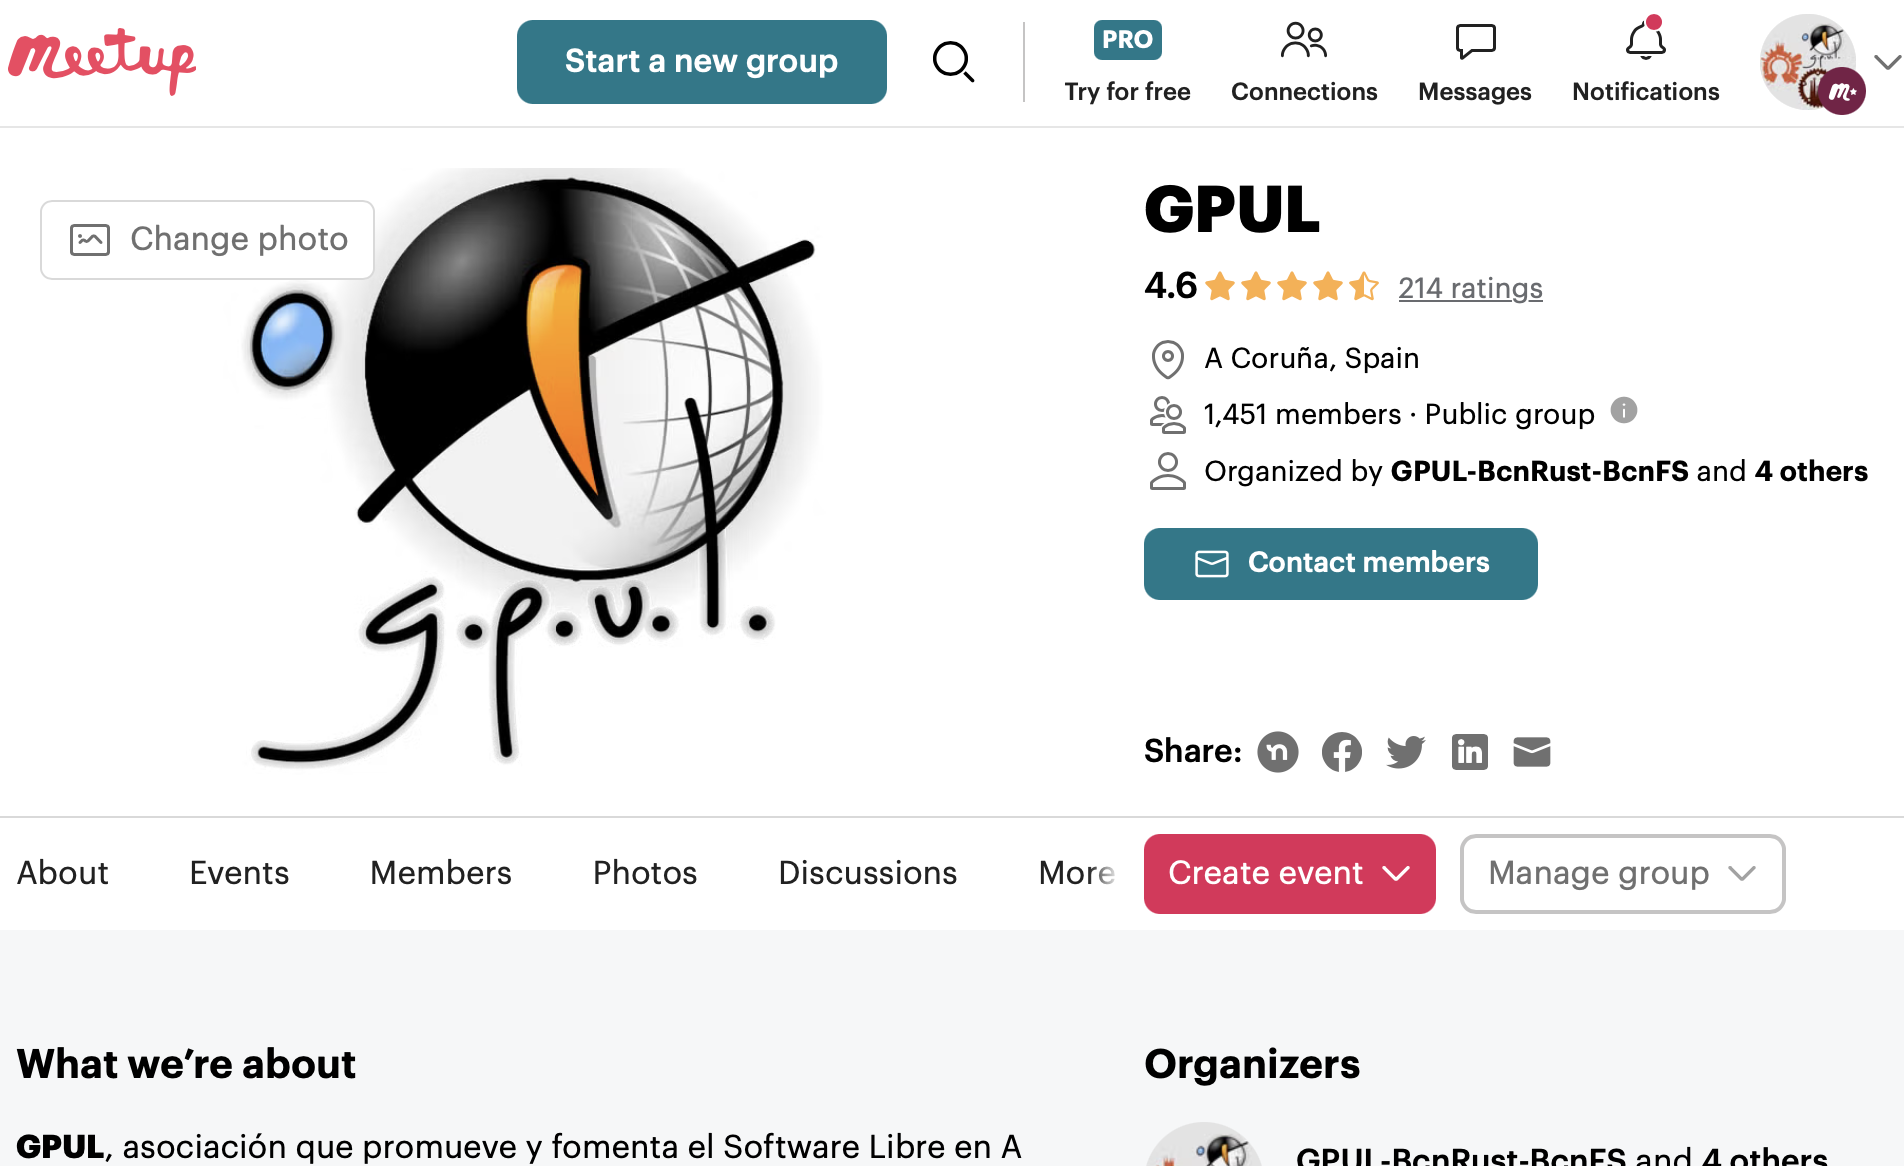
\includegraphics[width=0.9\textwidth]{imaxes/meetup-ui.png}
  \caption{Meetup interface}
  \label{fig:meetup-ui}
\end{figure}

\subsection*{pretalx}
\textbf{pretalx} is an open-source system for managing the full CFP process: submission, review, scheduling and communication. It allows custom submission forms, anonymous or public review workflows, and includes a schedule editor with conflict detection and speaker availability~\cite{pretalx-docs}. The software is written in Python (Django), supports plugins, and is licensed under Apache~2.0~\cite{pretalx-license}. A hosted service is also available for events that prefer not to self-host. A screenshot of the interface is shown in Figure~\ref{fig:pretalx-ui}.

\begin{figure}[H]
  \centering
  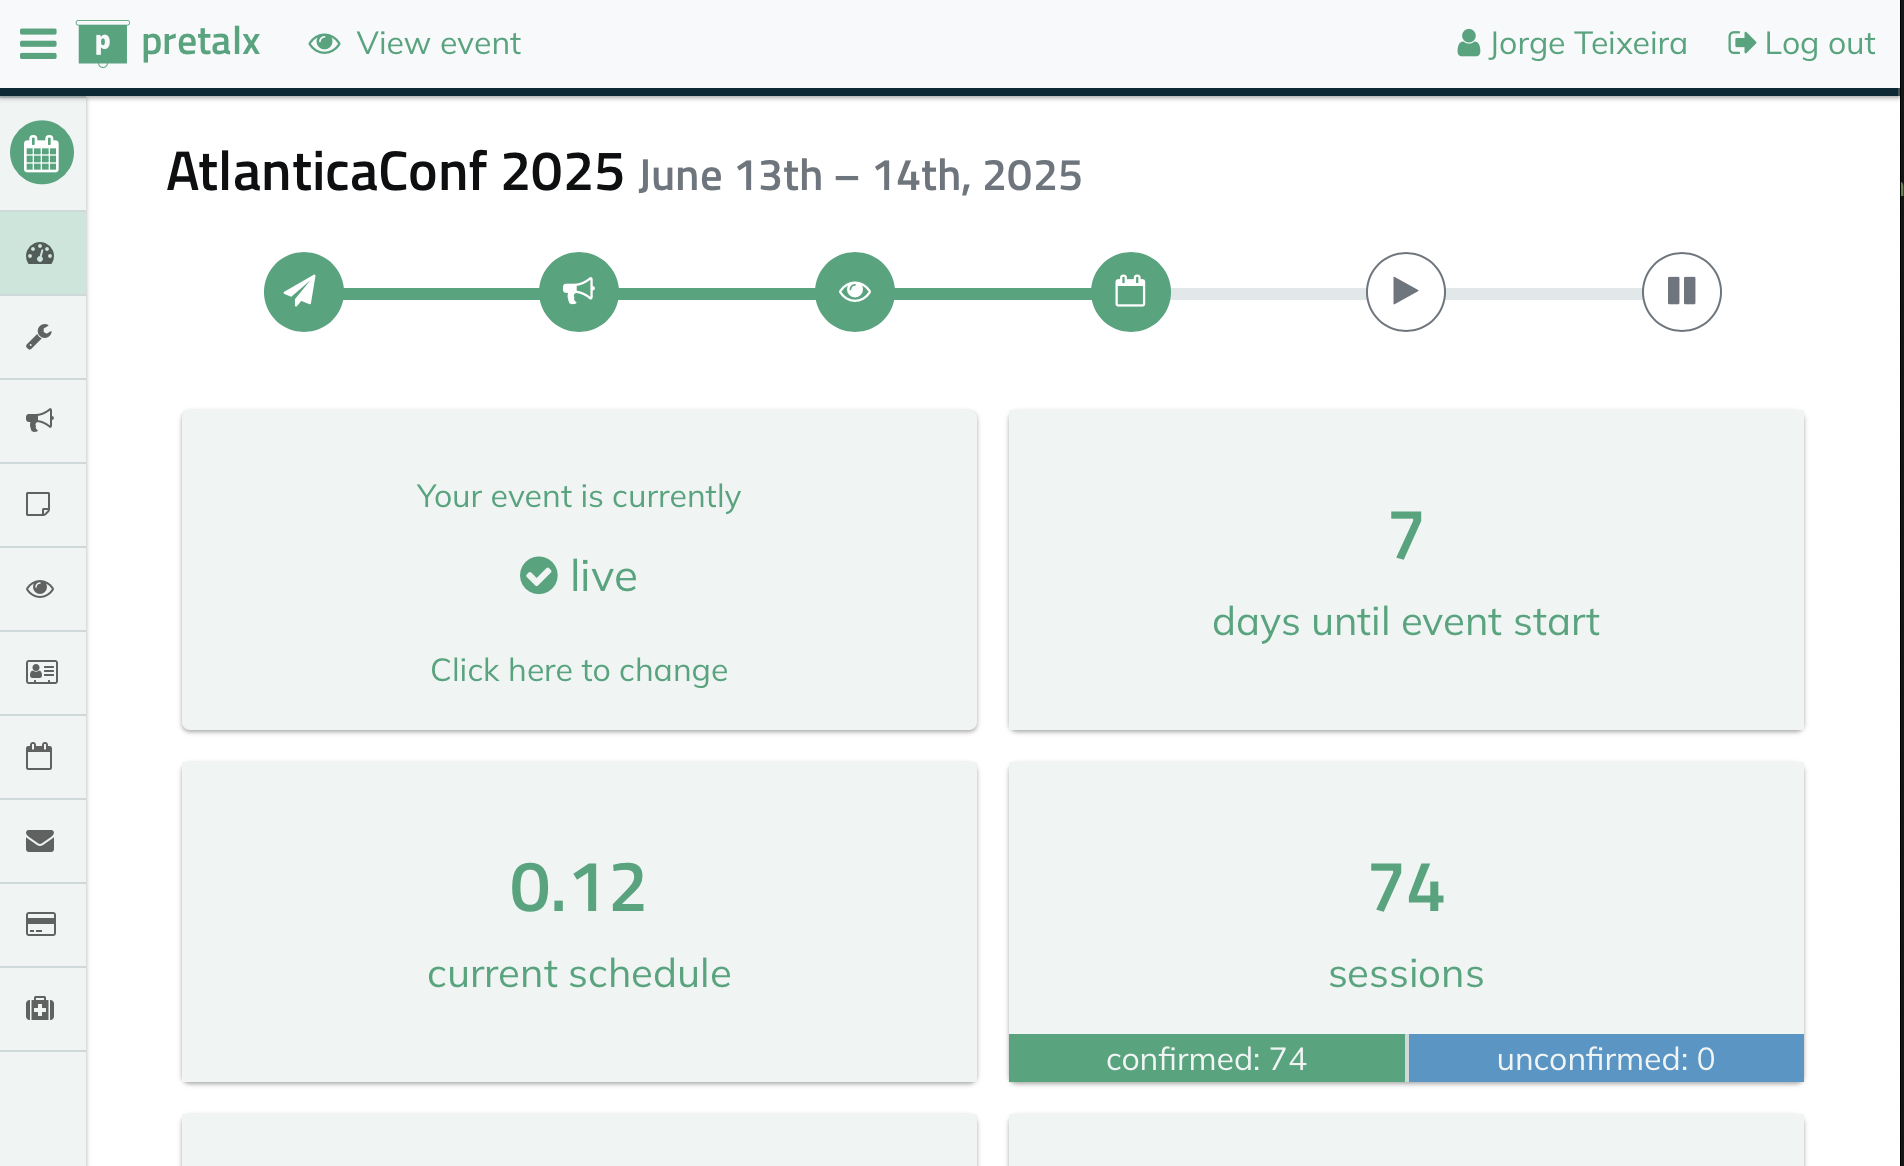
\includegraphics[width=0.9\textwidth]{imaxes/pretalx.com-ui.png}
  \caption{pretalx interface}
  \label{fig:pretalx-ui}
\end{figure}

\subsection*{pretix}
\textbf{pretix} is a feature-rich ticketing platform for events. It provides a configurable online shop, generates e-tickets, supports multiple payment gateways, and includes mobile apps for check-in~\cite{pretix-docs}. It is released under the AGPLv3 license and supports plugins for extensibility~\cite{pretix-license-faq}.

\subsection*{Koliseo}
\textbf{Koliseo} is an integrated open-source platform covering CFP, scheduling, and ticketing. It includes submission and agenda tools as well as QR-based ticketing using Stripe for payments. It is released under the Apache~2.0 license and offers a hosted version with a freemium model~\cite{koliseo-website}.

\subsection*{Indico}
\textbf{Indico}, developed at CERN, is a comprehensive event platform supporting abstracts, reviews, scheduling, registration, and badge printing. It is designed to scale and includes academic-focused features such as paper submissions and room booking~\cite{indico-github}. It is written in Python (Flask) and released under the MIT license~\cite{indico-faq}.

\subsection*{Proprietary Alternatives}
While this report focuses on open-source alternatives, GPUL currently relies on several proprietary services:

\begin{itemize}
  \item \textbf{Meetup}: Useful for visibility and community-building but limited in custom workflows. Organizers must pay a yearly subscription of around 200 €~\cite{meetup-wiki}.
  \item \textbf{Eventbrite}: Used for ticketing paid events. Charges a fee of around 10\% per ticket and does not support CFP~\cite{eventbrite-wiki}.
  \item \textbf{pretalx.com}: Hosted version of the open-source pretalx tool. Charges per event~\cite{pretalx-pricing}.
\end{itemize}

%--------------------------------------------------------------------
\section{Invoicing / Accounting}

\textbf{Importance.} Compliant invoicing and accounting are a legal necessity for any formally constituted association, governed by national and regional regulations. This is a particularly pressing issue in Spain, where upcoming \textbf{VeriFactu} regulations will mandate certified electronic invoicing systems that report to the tax agency (AEAT) in real-time. For GPUL, abandoning manual, non-compliant methods is not merely an upgrade but a mandatory step to ensure legal and fiscal viability \cite{odoo-blog-verifactu}.

\subsection*{Current stack}
LibreOffice templates stored in Nextcloud, with manual PDF generation and signing. No Facturae, XML or AEAT compliance is currently met. A screenshot of the current invoice template is shown in Figure~\ref{fig:invoice}.

\begin{figure}[H]
  \centering
  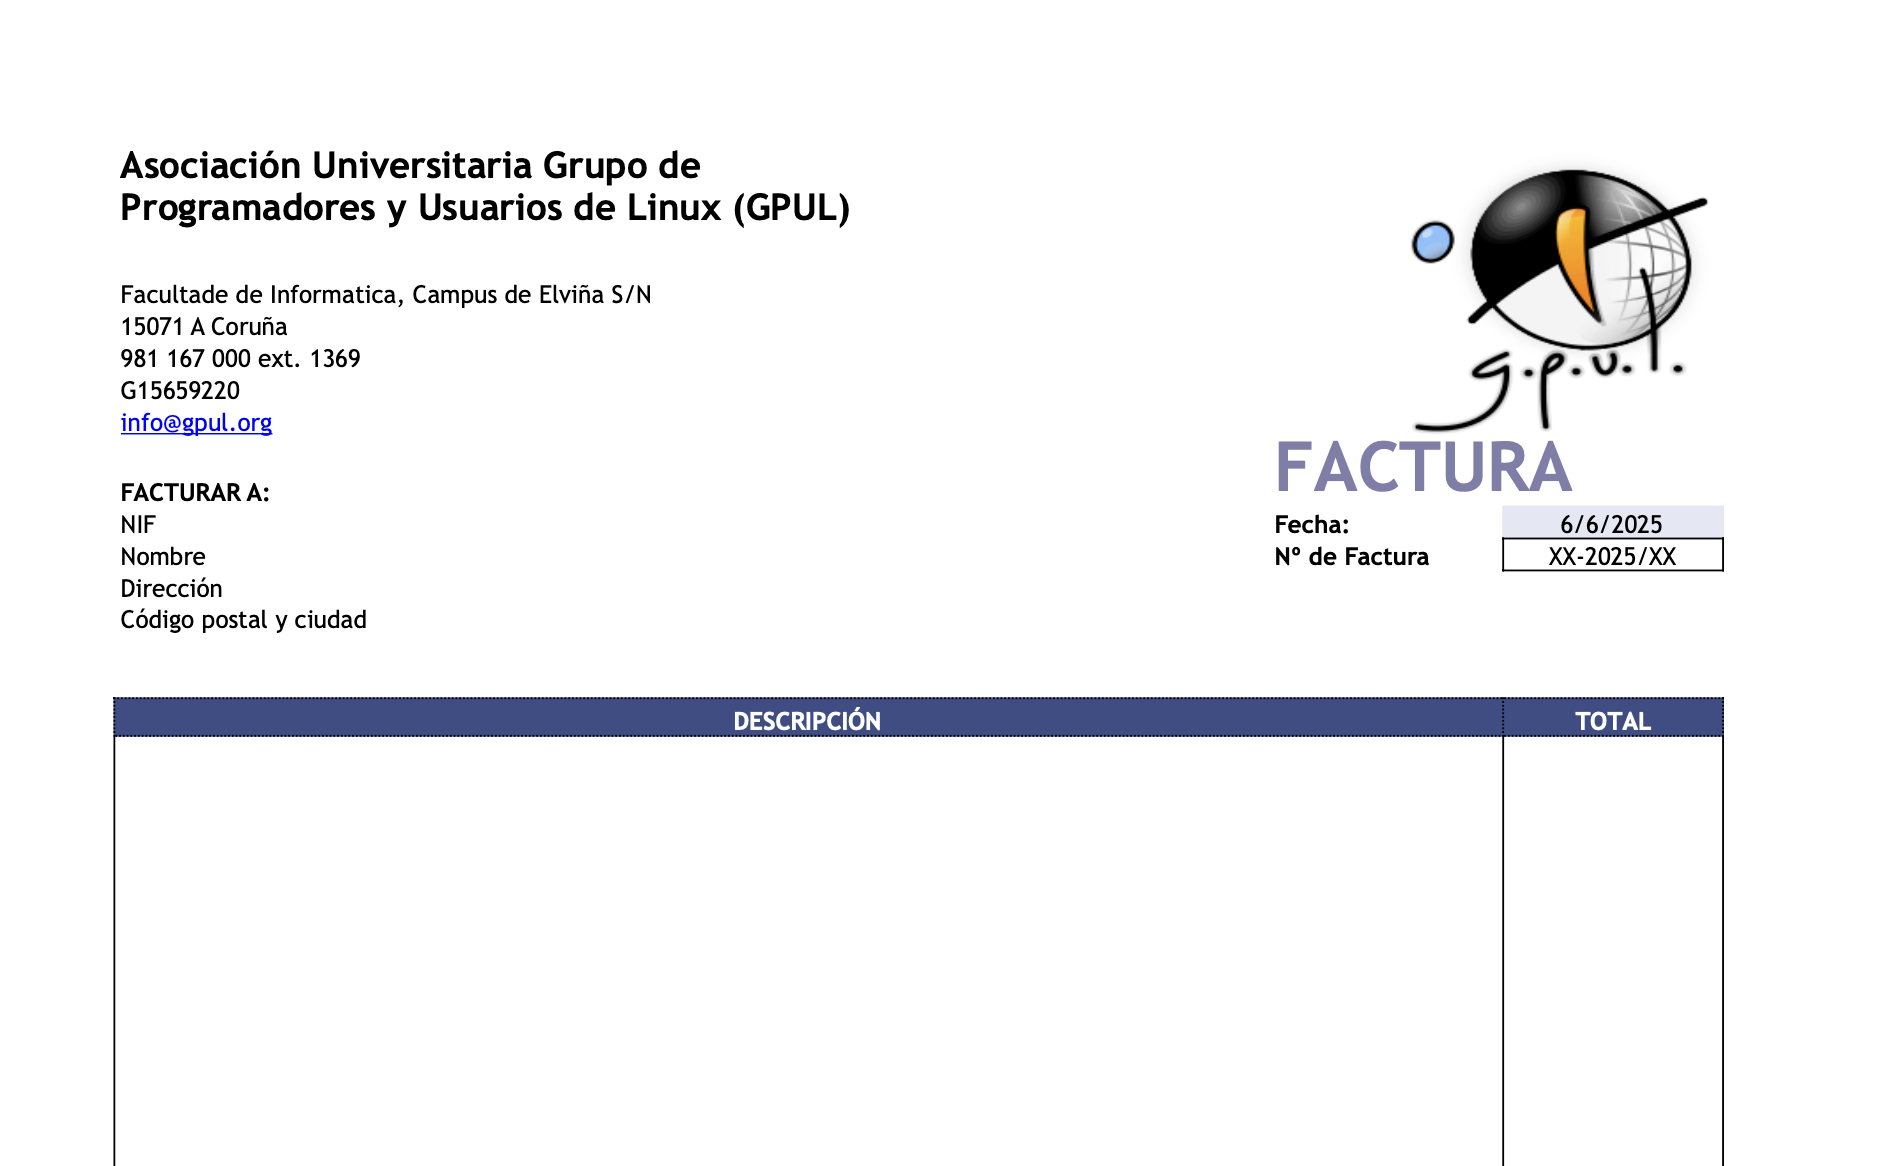
\includegraphics[width=0.9\textwidth]{imaxes/invoice.png}
  \caption{Current invoice template}
  \label{fig:invoice}
\end{figure}

\subsection*{Odoo}
Full ERP with accounting and invoicing modules. Spanish localization modules allow Facturae XML export, AEAT integration, SII support and planned VeriFactu readiness \cite{odoo-einvoice-spain}. Heavy stack and learning curve, but suitable for full integration. A screenshot of the interface is shown in Figure~\ref{fig:odoo-ui}.

\begin{figure}[H]
  \centering
  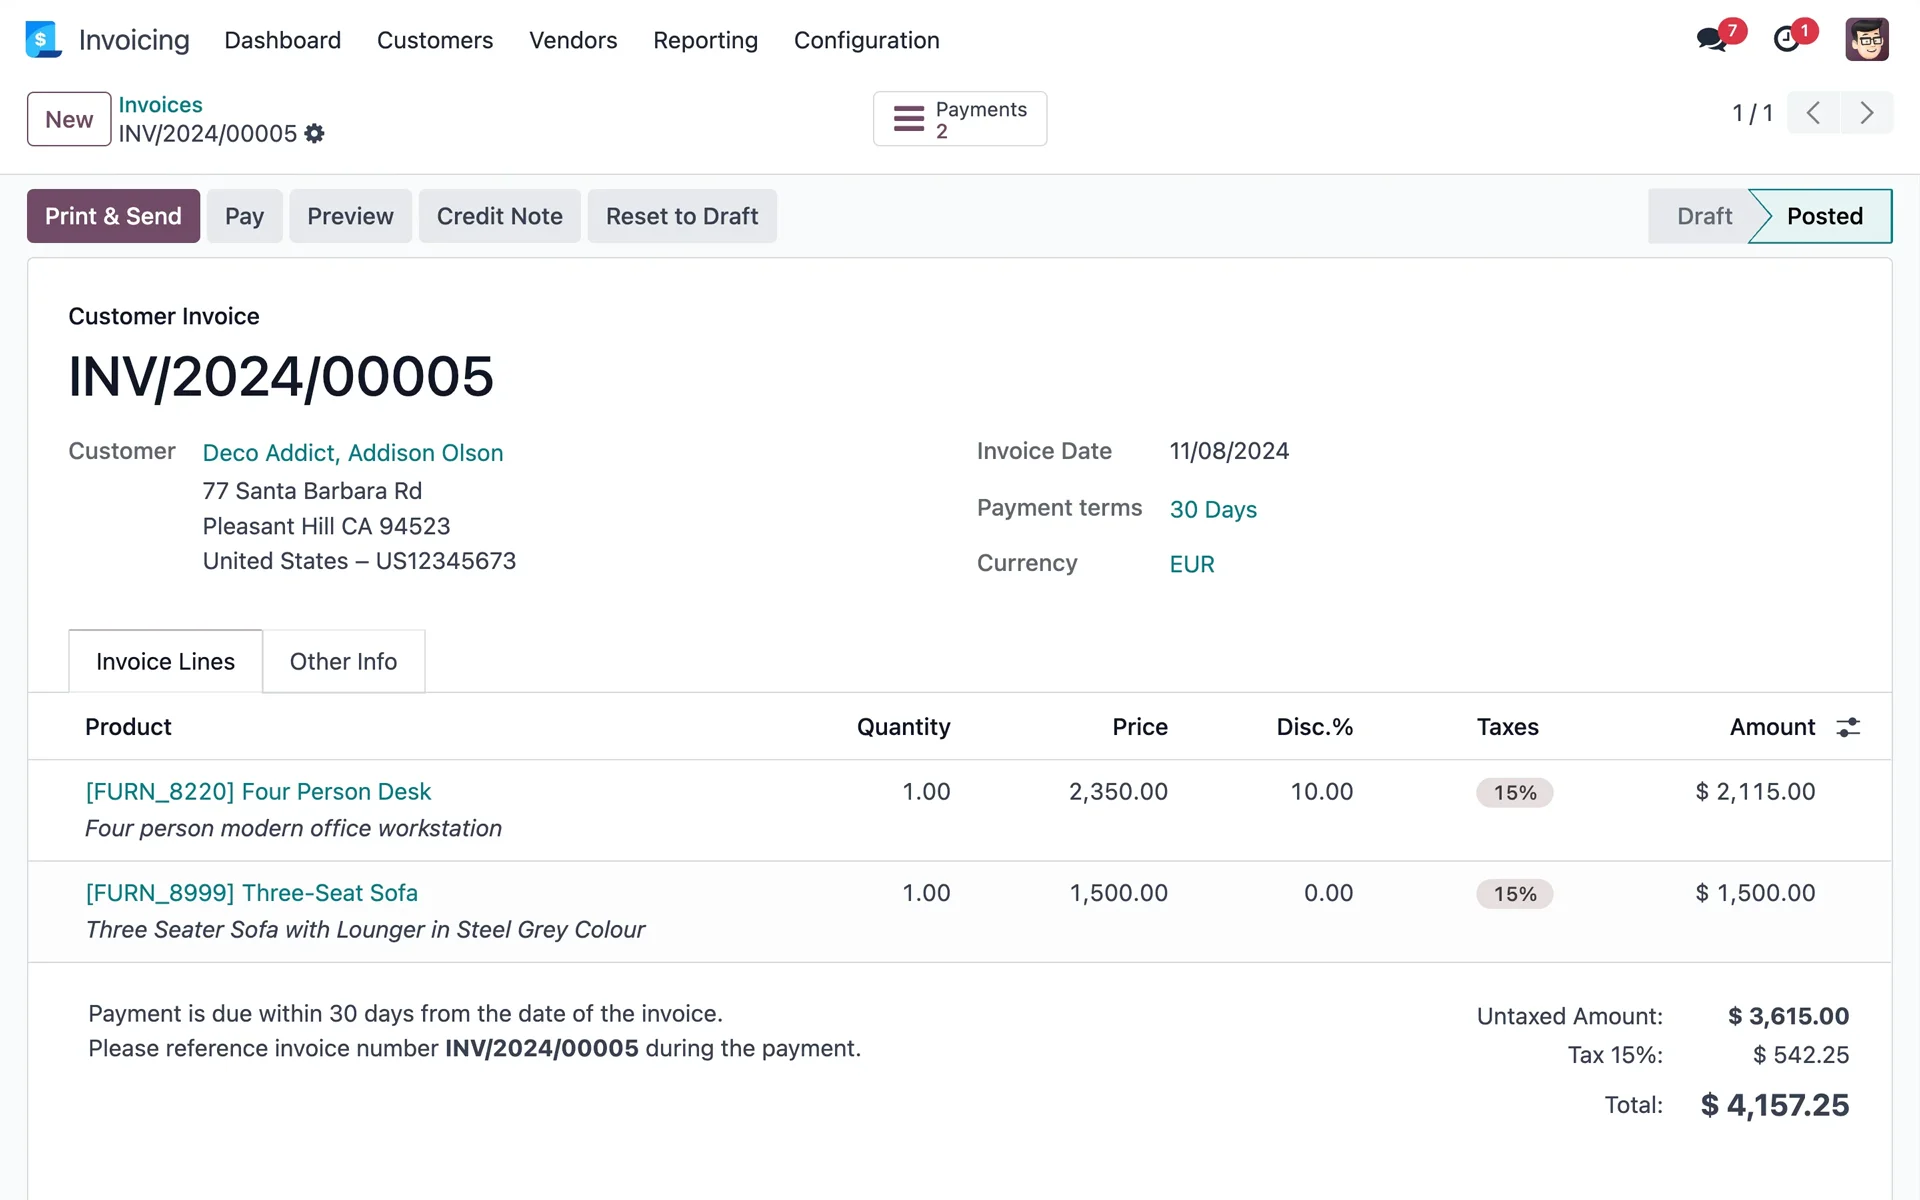
\includegraphics[width=0.9\textwidth]{imaxes/odoo-ui.png}
  \caption{Odoo interface}
  \label{fig:odoo-ui}
\end{figure}

\subsection*{FacturaScripts}
Spanish-made open source ERP with strong native support for Facturae and IRPF/IVA reporting. Plugin system allows automatic signing and XML export \cite{facturascripts-antifraude}. VeriFactu modules planned by maintainers. A screenshot of the interface is shown in Figure~\ref{fig:facturascripts-ui}.

\begin{figure}[H]
  \centering
  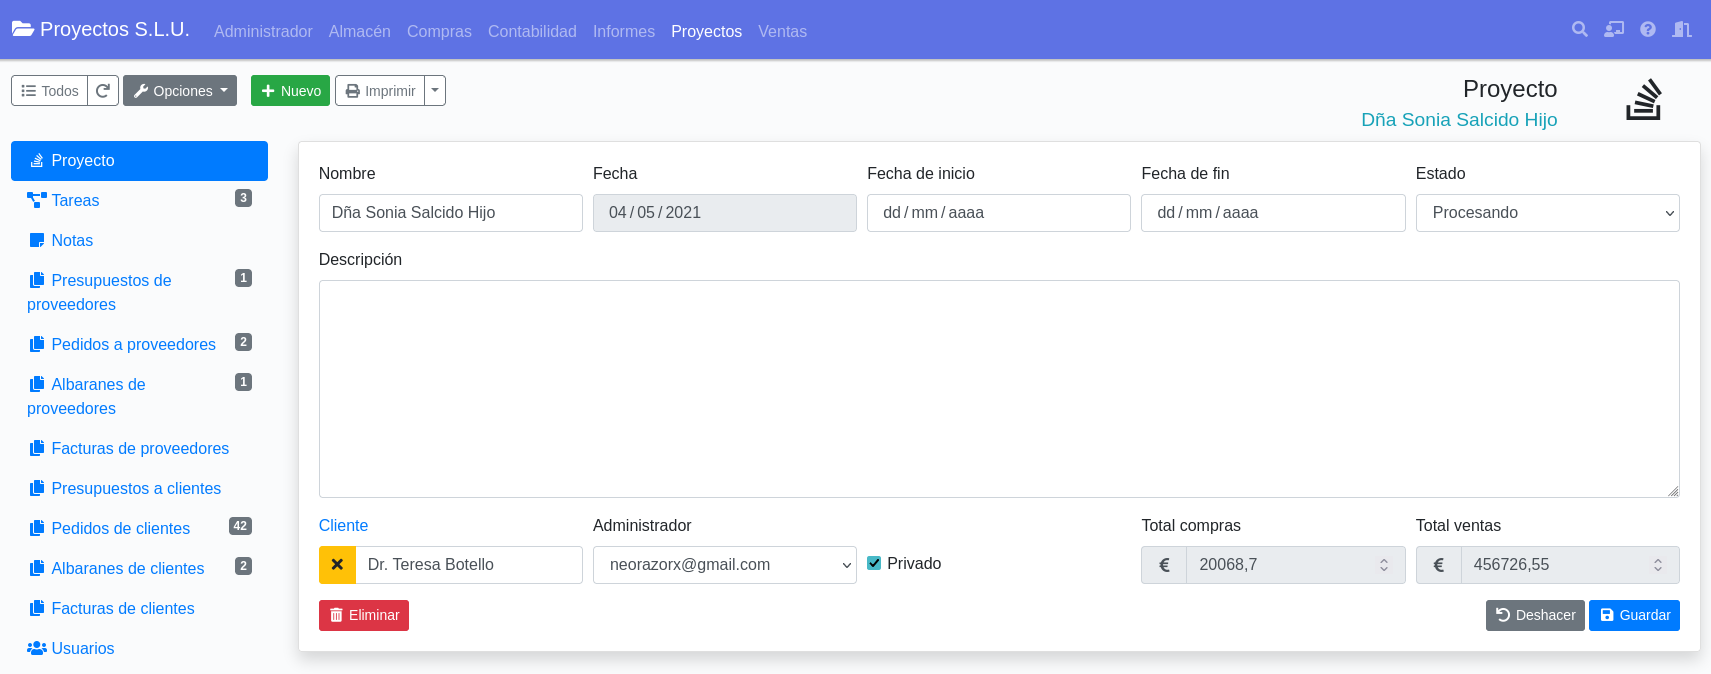
\includegraphics[width=0.9\textwidth]{imaxes/facturascripts-ui.png}
  \caption{FacturaScripts interface}
  \label{fig:facturascripts-ui}
\end{figure}

\subsection*{Proprietary Alternatives}

\textbf{Holded} and \textbf{Quipu} are both popular Spanish cloud ERPs with direct AEAT and VeriFactu compliance out of the box \cite{holded-verifactu}. \textbf{Sage} offers several solutions (Sage 50, Sage Despachos) and promotes VeriFactu-compliant accountant platforms \cite{sage-verifactu}.

\subsection*{External Accountant}
A viable route is outsourcing invoice issuance and reporting through a accounting firm. Most use certified tools (e.g., Sage) and provide invoice portals. This model outsources technical complexity and ensures compliance, but implies higher cost and less internal control \cite{sage-blog-asesoria}.

%--------------------------------------------------------------------
\section{Phone / VoIP Integration}

\textbf{Importance.} While not essential for every organization, integrating a physical phone line with a VoIP system can solve key accessibility challenges. It allows calls to be managed remotely, ensuring continuity even when no one is physically present at an office. For GPUL, the university provides a physical phone extension in its office. Integrating this line into a digital system would make it possible to receive and route calls remotely, transforming a location-dependent asset into a flexible communication tool for the whole team.

\subsection*{Current stack}

A standard analog line is connected to a desk phone in the office, routed internally from the university's telephony system. There is currently no digital or remote integration.

\subsection*{Analog to VoIP Integration}

To interface analog phone lines with VoIP systems, \gls{fxo} gateways or cards are used. \gls{fxo} interfaces connect to analog lines (e.g., from the wall), converting them to VoIP (typically \gls{sip}) for use by a \gls{pbx}. Conversely, \gls{fxs} interfaces allow analog phones to connect to VoIP systems \cite{yeastar-fxo-fxs-2024}.

\begin{figure}[H]
  \centering
  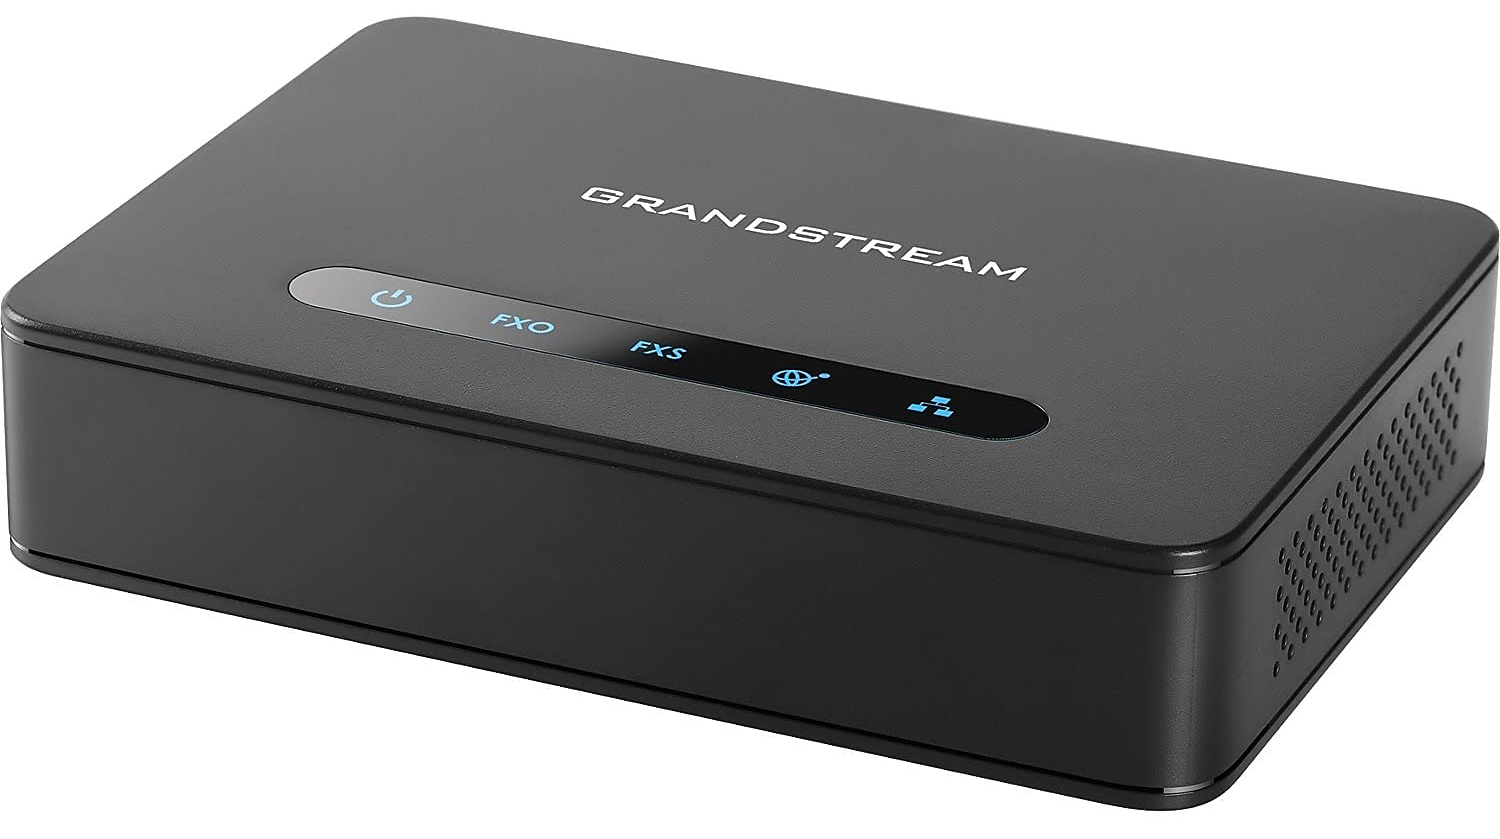
\includegraphics[width=0.7\textwidth]{imaxes/grandstream-ht.png}
  \caption{Grandstream HT813}
  \label{fig:grandstream-ht}
\end{figure}

Typical setups use Ethernet-based FXO gateways like the Grandstream HT (Figure~\ref{fig:grandstream-ht}) series or Yeastar TA series, which register as trunks to a VoIP server such as Asterisk or 3CX. These enable both incoming and outgoing call routing using the existing line while allowing softphone clients (desktop, mobile) to act as remote extensions \cite{yeastar-fxo-fxs-2024}.

\subsection*{Asterisk + FreePBX}

Asterisk is a mature open-source \gls{pbx} capable of managing analog and SIP trunks, extensions, voicemail, IVRs, and more. When combined with a GUI like FreePBX or Issabel, it becomes easier to configure and deploy. A screenshot of the FreePBX interface is shown in Figure~\ref{fig:freepbx-ui}.

\begin{figure}[H]
  \centering
  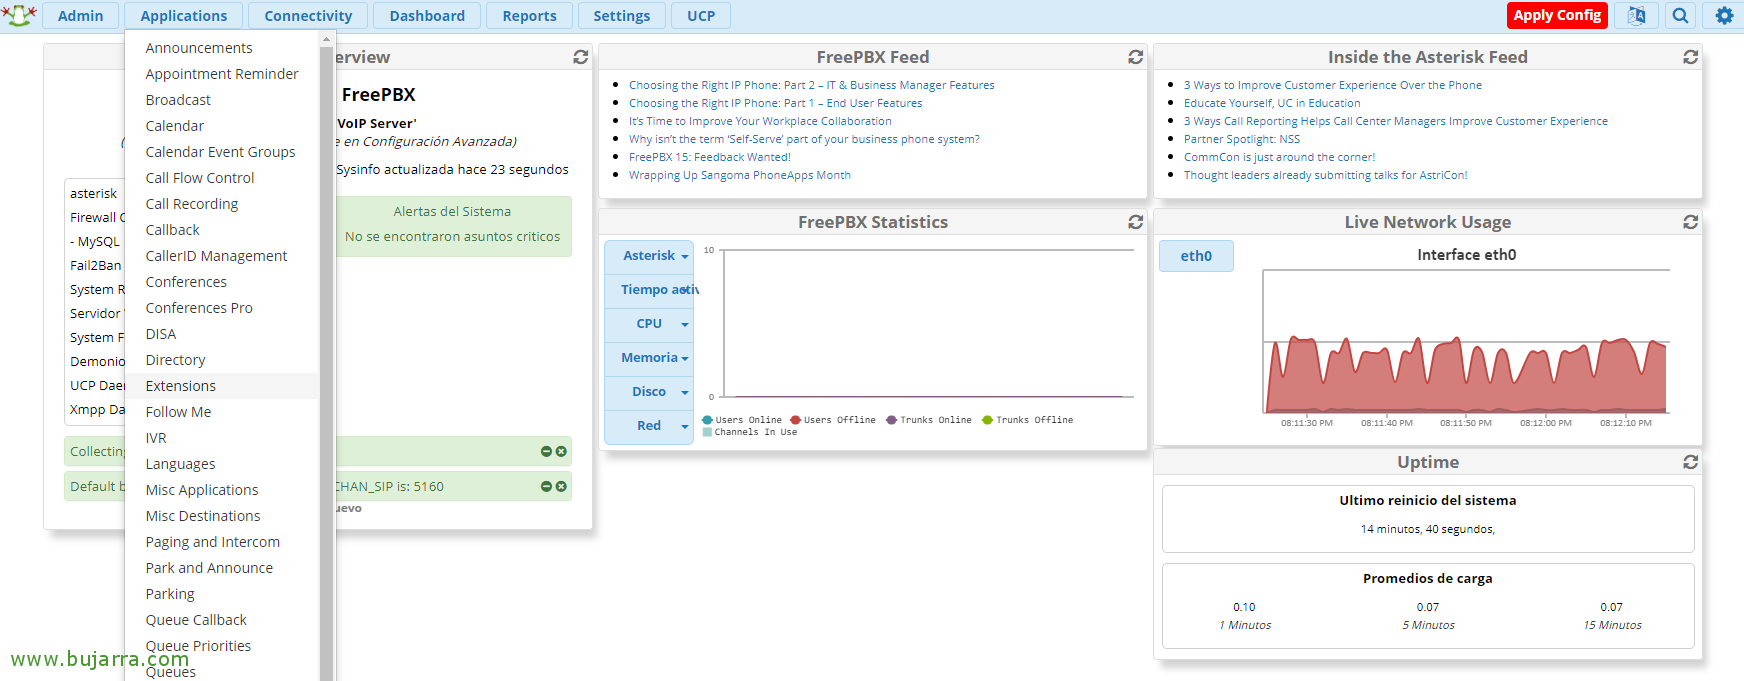
\includegraphics[width=0.9\textwidth]{imaxes/freepbx-ui.png}
  \caption{FreePBX interface}
  \label{fig:freepbx-ui}
\end{figure}

Voicemail-to-email and softphone integration are supported. Hardware support includes both PCI FXO cards and SIP-registered gateways \cite{asterisk-features}.
\subsection*{Softphones and Mobile Integration}

Modern PBXs support softphones via \gls{sip}, enabling remote call management. Tools like Zoiper, Linphone, and Jitsi are compatible with both Asterisk and 3CX, and can register as \gls{sip} extensions. 3CX also provides native apps with push notifications and browser-based calling \cite{zoiper-compatibility}.

\subsection*{Proprietary Alternatives}

3CX is a proprietary VoIP platform with a free on-premise edition for up to 10 users. It includes native apps for iOS, Android, desktop, and web. Configuration is GUI-based and generally more user-friendly than raw Asterisk. While closed-source, it offers an integrated, modern stack with mobile push notifications, video calls, and softphone provisioning \cite{3cx-pricing-2024}. FXO gateways are supported as SIP trunks, enabling analog line integration similar to Asterisk. A screenshot of the 3CX interface is shown in Figure~\ref{fig:3cx-ui}.

\begin{figure}[H]
  \centering
  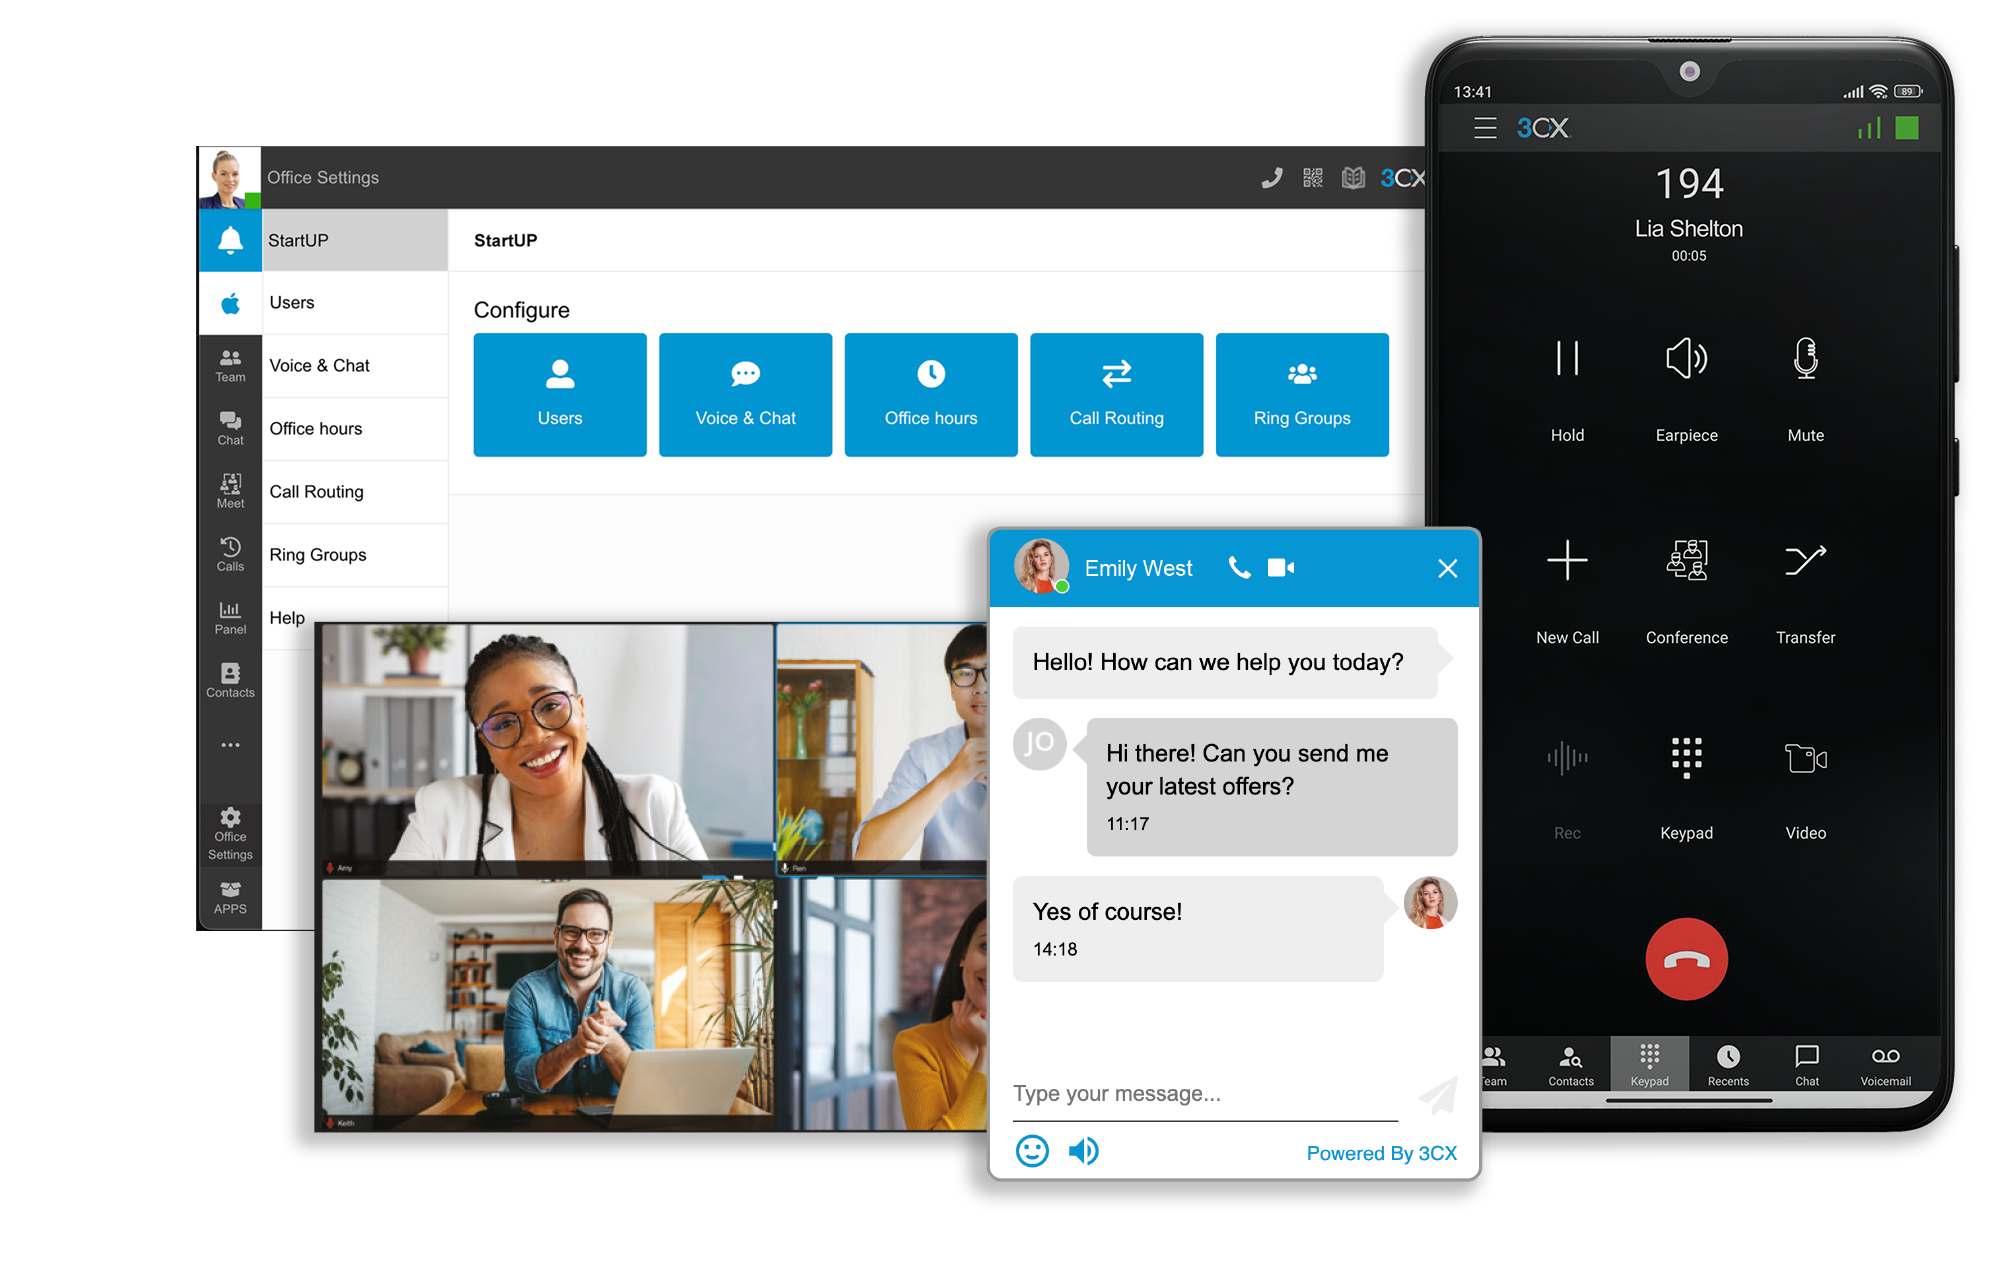
\includegraphics[width=0.9\textwidth]{imaxes/3cx-ui.png}
  \caption{3CX interface}
  \label{fig:3cx-ui}
\end{figure}

Other platforms like Cisco Webex Calling or Zoom Phone offer similar capabilities but are not open source and come with usage-based pricing. These are not explored further here due to the self-hosting and sovereignty focus of this document.

\section{Service Deployment and Management}

\textbf{Importance.} A reliable and reproducible deployment workflow is crucial for the long-term sustainability of any technical infrastructure, especially one managed by volunteers. It ensures that services can be easily replicated, recovered from failures, and maintained by future members. For GPUL, the current mix of bare-metal and manual container deployments is fragile and poorly documented. Adopting a modern virtualization or orchestration platform is essential to create a resilient, scalable, and manageable infrastructure for the future.

\subsection*{Current stack}
The current infrastructure consists of a mixture of services deployed directly on bare metal and others managed via \texttt{docker-compose}, spread across two physical servers. There is no centralized management layer, which complicates monitoring, scaling, and service replication. Containers are started manually, with limited documentation or automation.

\subsection*{Proxmox VE}

Proxmox Virtual Environment (VE) is an open-source virtualization management platform (Debian-based) that integrates KVM-based virtual machines and LXC containers \cite{proxmox-admin-guide-2025}. It provides a unified web-based interface and CLI for creating and managing VMs and containers, aiming for ease of administration so that even novices can deploy it within minutes . Proxmox can run on a single server or in a multi-node cluster (with a multi-master design and a clustered filesystem) to enable high availability and live migration of workloads . It supports flexible storage backends (local or shared storage) and includes a fully integrated backup/restore solution (via Proxmox Backup Server or vzdump) for protecting VM and container data . These features make Proxmox suitable for self-hosted labs needing a mix of VM and container workloads managed in a unified open-source platform. A screenshot of the interface is shown in Figure~\ref{fig:proxmox-ui}.

\begin{figure}[H]
  \centering
  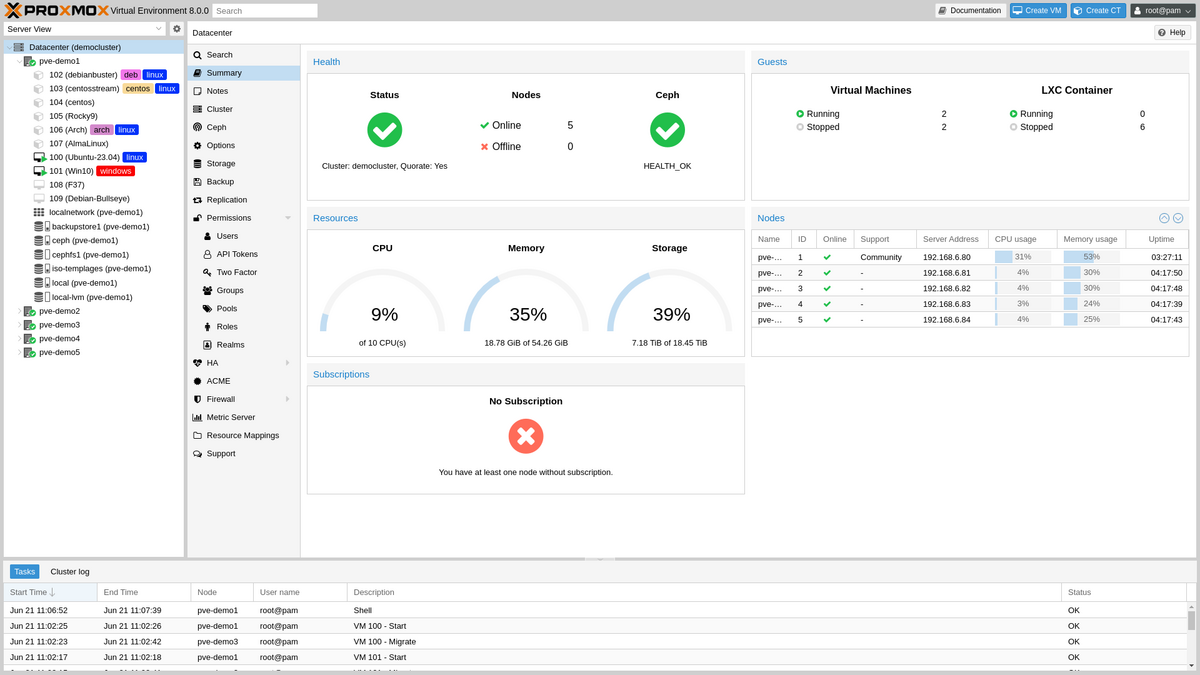
\includegraphics[width=0.9\textwidth]{imaxes/proxmox-ui.png}
  \caption{Proxmox interface}
  \label{fig:proxmox-ui}
\end{figure}

\subsection*{Incus (LXD)}

Incus is a modern open-source container and VM manager (a fork of LXD) that provides a cloud-like experience on Linux hosts \cite{incus-linux-containers-2023}. It is image-based and supports a wide range of Linux distributions, providing both system containers (sharing the host kernel) and application containers, as well as full virtual machines with guest kernels . Incus uses a single command-line tool and REST API for local or remote management of instances, with features like snapshots, live migration, and resource profiling. It is designed to scale from a single node up to large clusters (thousands of servers)  and works on any recent Linux distribution (packages available via various distros) . In practice, Incus is used for lightweight virtualization on commodity hardware, where administrators want to mix containers and VMs with relatively low overhead and a straightforward CLI/API interface.

\subsection*{Docker and Podman}

Docker and Podman are containerization platforms for running applications in isolated environments. Docker (Docker Engine) popularized this approach by packaging code and dependencies into portable containers \cite{spacelift-podman-docker-2024}. It follows a daemon-based model and supports layered images and declarative Dockerfiles. Docker also provides Docker Compose for defining multi-container applications via a single YAML file and (historically) a Swarm mode for basic clustering and service replication . Podman is a daemonless, rootless container engine (a drop-in Docker replacement) that runs containers as child processes of the user, improving security isolation . Podman supports most Docker CLI commands and introduces "pods" (groups of containers sharing the same network namespace) similar to Kubernetes pods . For orchestration, Docker relies on Docker Compose and Swarm, whereas Podman can use \texttt{podman-compose} or generate Kubernetes manifests; Podman itself has no built-in high-availability orchestrator . Podman is often favored in security-sensitive or multi-user environments (and is default on many Linux distributions), while Docker remains widely used in development and CI/CD environments due to its mature ecosystem and tools .

\subsection*{Kubernetes}

Kubernetes is an open-source container orchestration system originally developed by Google \cite{kubernetes-docs-2025}. It automates deployment, scaling, and management of containerized applications. Kubernetes groups containers into logical units called \emph{pods} (each pod contains one or more containers with shared storage and networking) . A Kubernetes cluster typically includes multiple control-plane (master) and worker nodes; users define desired application state via declarative manifests (Deployments, Services, etc.), and Kubernetes automatically schedules pods onto nodes. The platform handles service discovery, load balancing, rolling updates/rollbacks, and self-healing (restarting failed containers) . It "provides a framework to run distributed systems resiliently," automatically handling scaling, failover, and automated rollouts . Kubernetes also supports secrets/config management and horizontal pod autoscaling. However, Kubernetes has substantial operational complexity and resource requirements. For small-scale setups, lightweight distributions like k3s or MicroK8s strip out legacy components to simplify installation and reduce footprint, making Kubernetes feasible even for edge or two-node deployments \cite{k3s-microk8s-2022}. In summary, Kubernetes excels in orchestrating multi-host container clusters with advanced features, whereas simpler tools (like Docker Compose or single-node Incus/Proxmox) may suffice for smaller self-hosted environments.

\subsection*{Proprietary Alternatives}

There are several proprietary platforms offering infrastructure orchestration and service management, such as VMware vSphere, Red Hat OpenShift, and Amazon ECS. However, in this particular domain, open-source solutions are not only mature and widely adopted, but also provide superior flexibility, transparency, and long-term maintainability. As such, proprietary tools are not considered viable contenders for the association's use case.
